
\section{Caracterizaci\'on}

Siguiendo el trabajo de \citet{zotenko2008} tomamos cuatro redes de interacci\'on de levadura (\textit{Saccharomyces cerevisiae}) disponibles en el Yeast Interactome Database\footnote{http://interactome.dfci.harvard.edu/S\_cerevisiae/}. Estas redes fueron obtenidas a partir de diferentes t\'ecnicas: a trav\'es de Affinity-Purification/Mass-Spectrometry (AP-MS) \citep{apms_data}; de 
interacciones binarias Yeast Two-Hybrid (Y2H) \citep{y2h_data} y dos curadas de literatura \citep{lit_data} {\bf (FALTA UNA CITA AQUI)}. La figura \ref{grafos} muestra una representaci\'on gr\'afica de las cuatro redes consideradas.


% La idea del ejercicio es realizar un analisis cuantitativo de las tres redes y observar las coherencia entre las interacciones reportadas


\begin{figure}[!ht]
    \centering
    \begin{subfigure}[b]{0.4\columnwidth}
        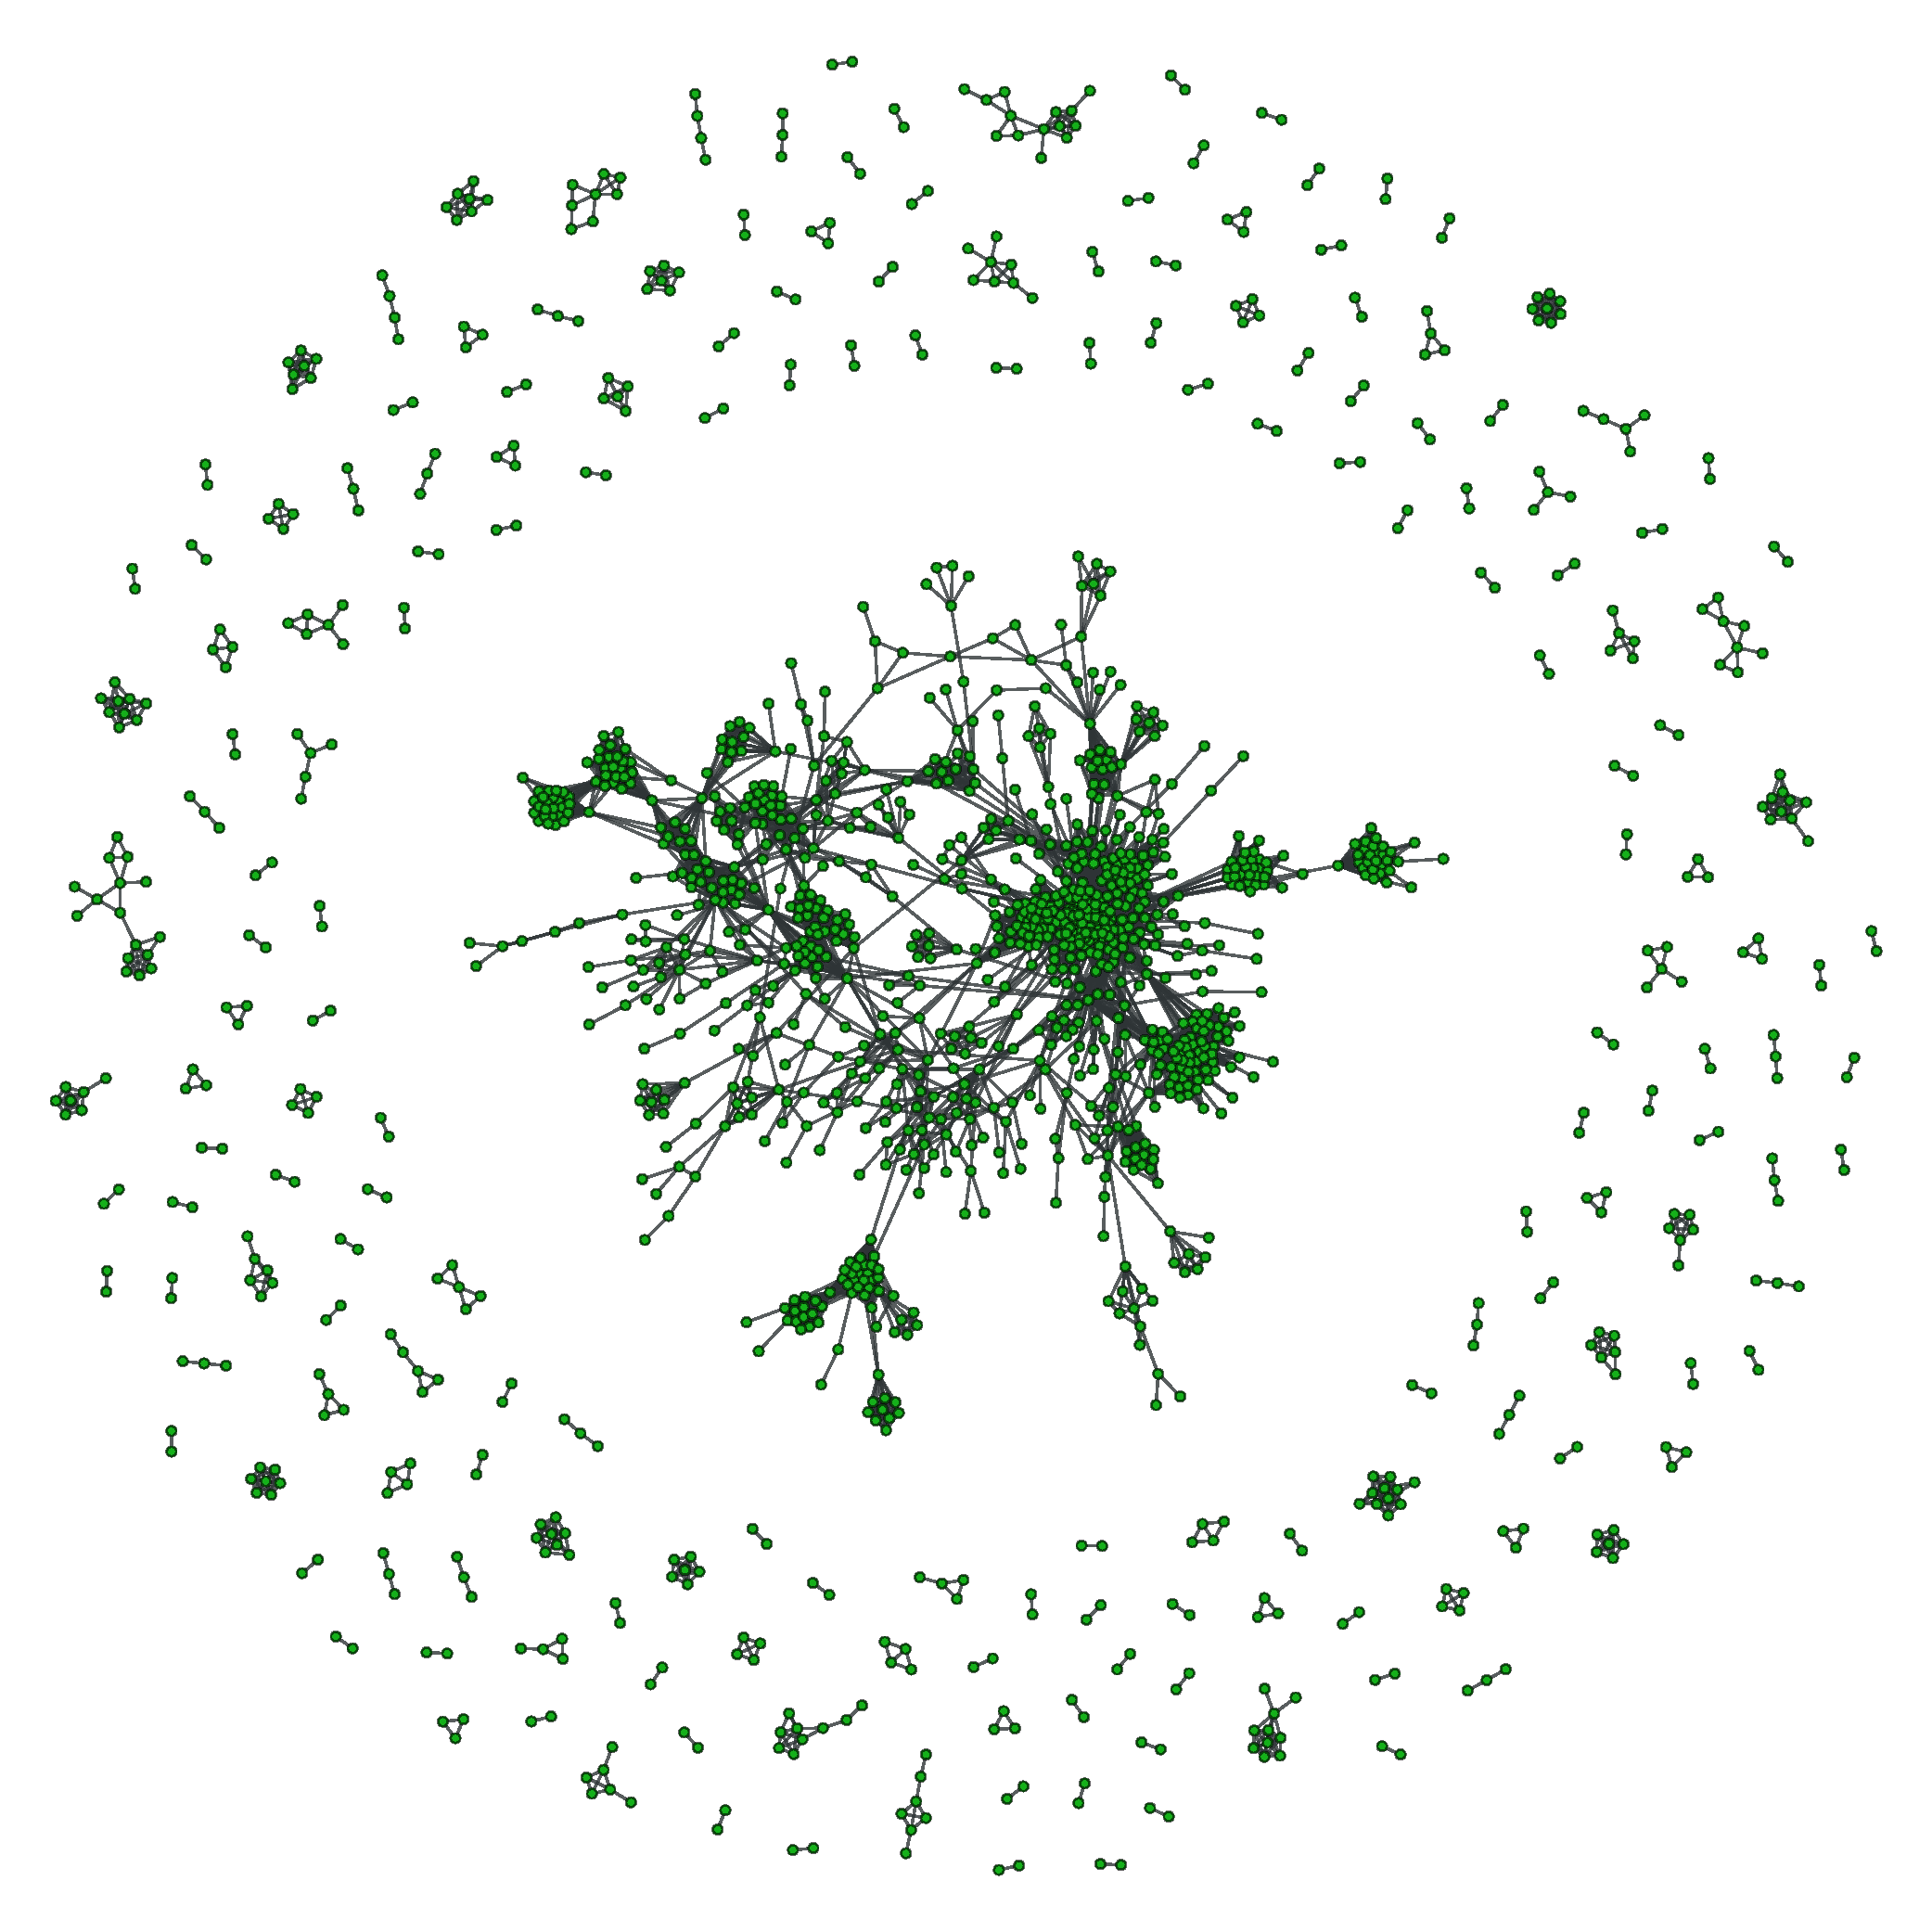
\includegraphics[width=\textwidth]{./schemes/yeast_AP-MS-txt.pdf}
        \caption{\label{fig:ap_ms} AP-MS}
    \end{subfigure}
    \begin{subfigure}[b]{0.4\columnwidth}
        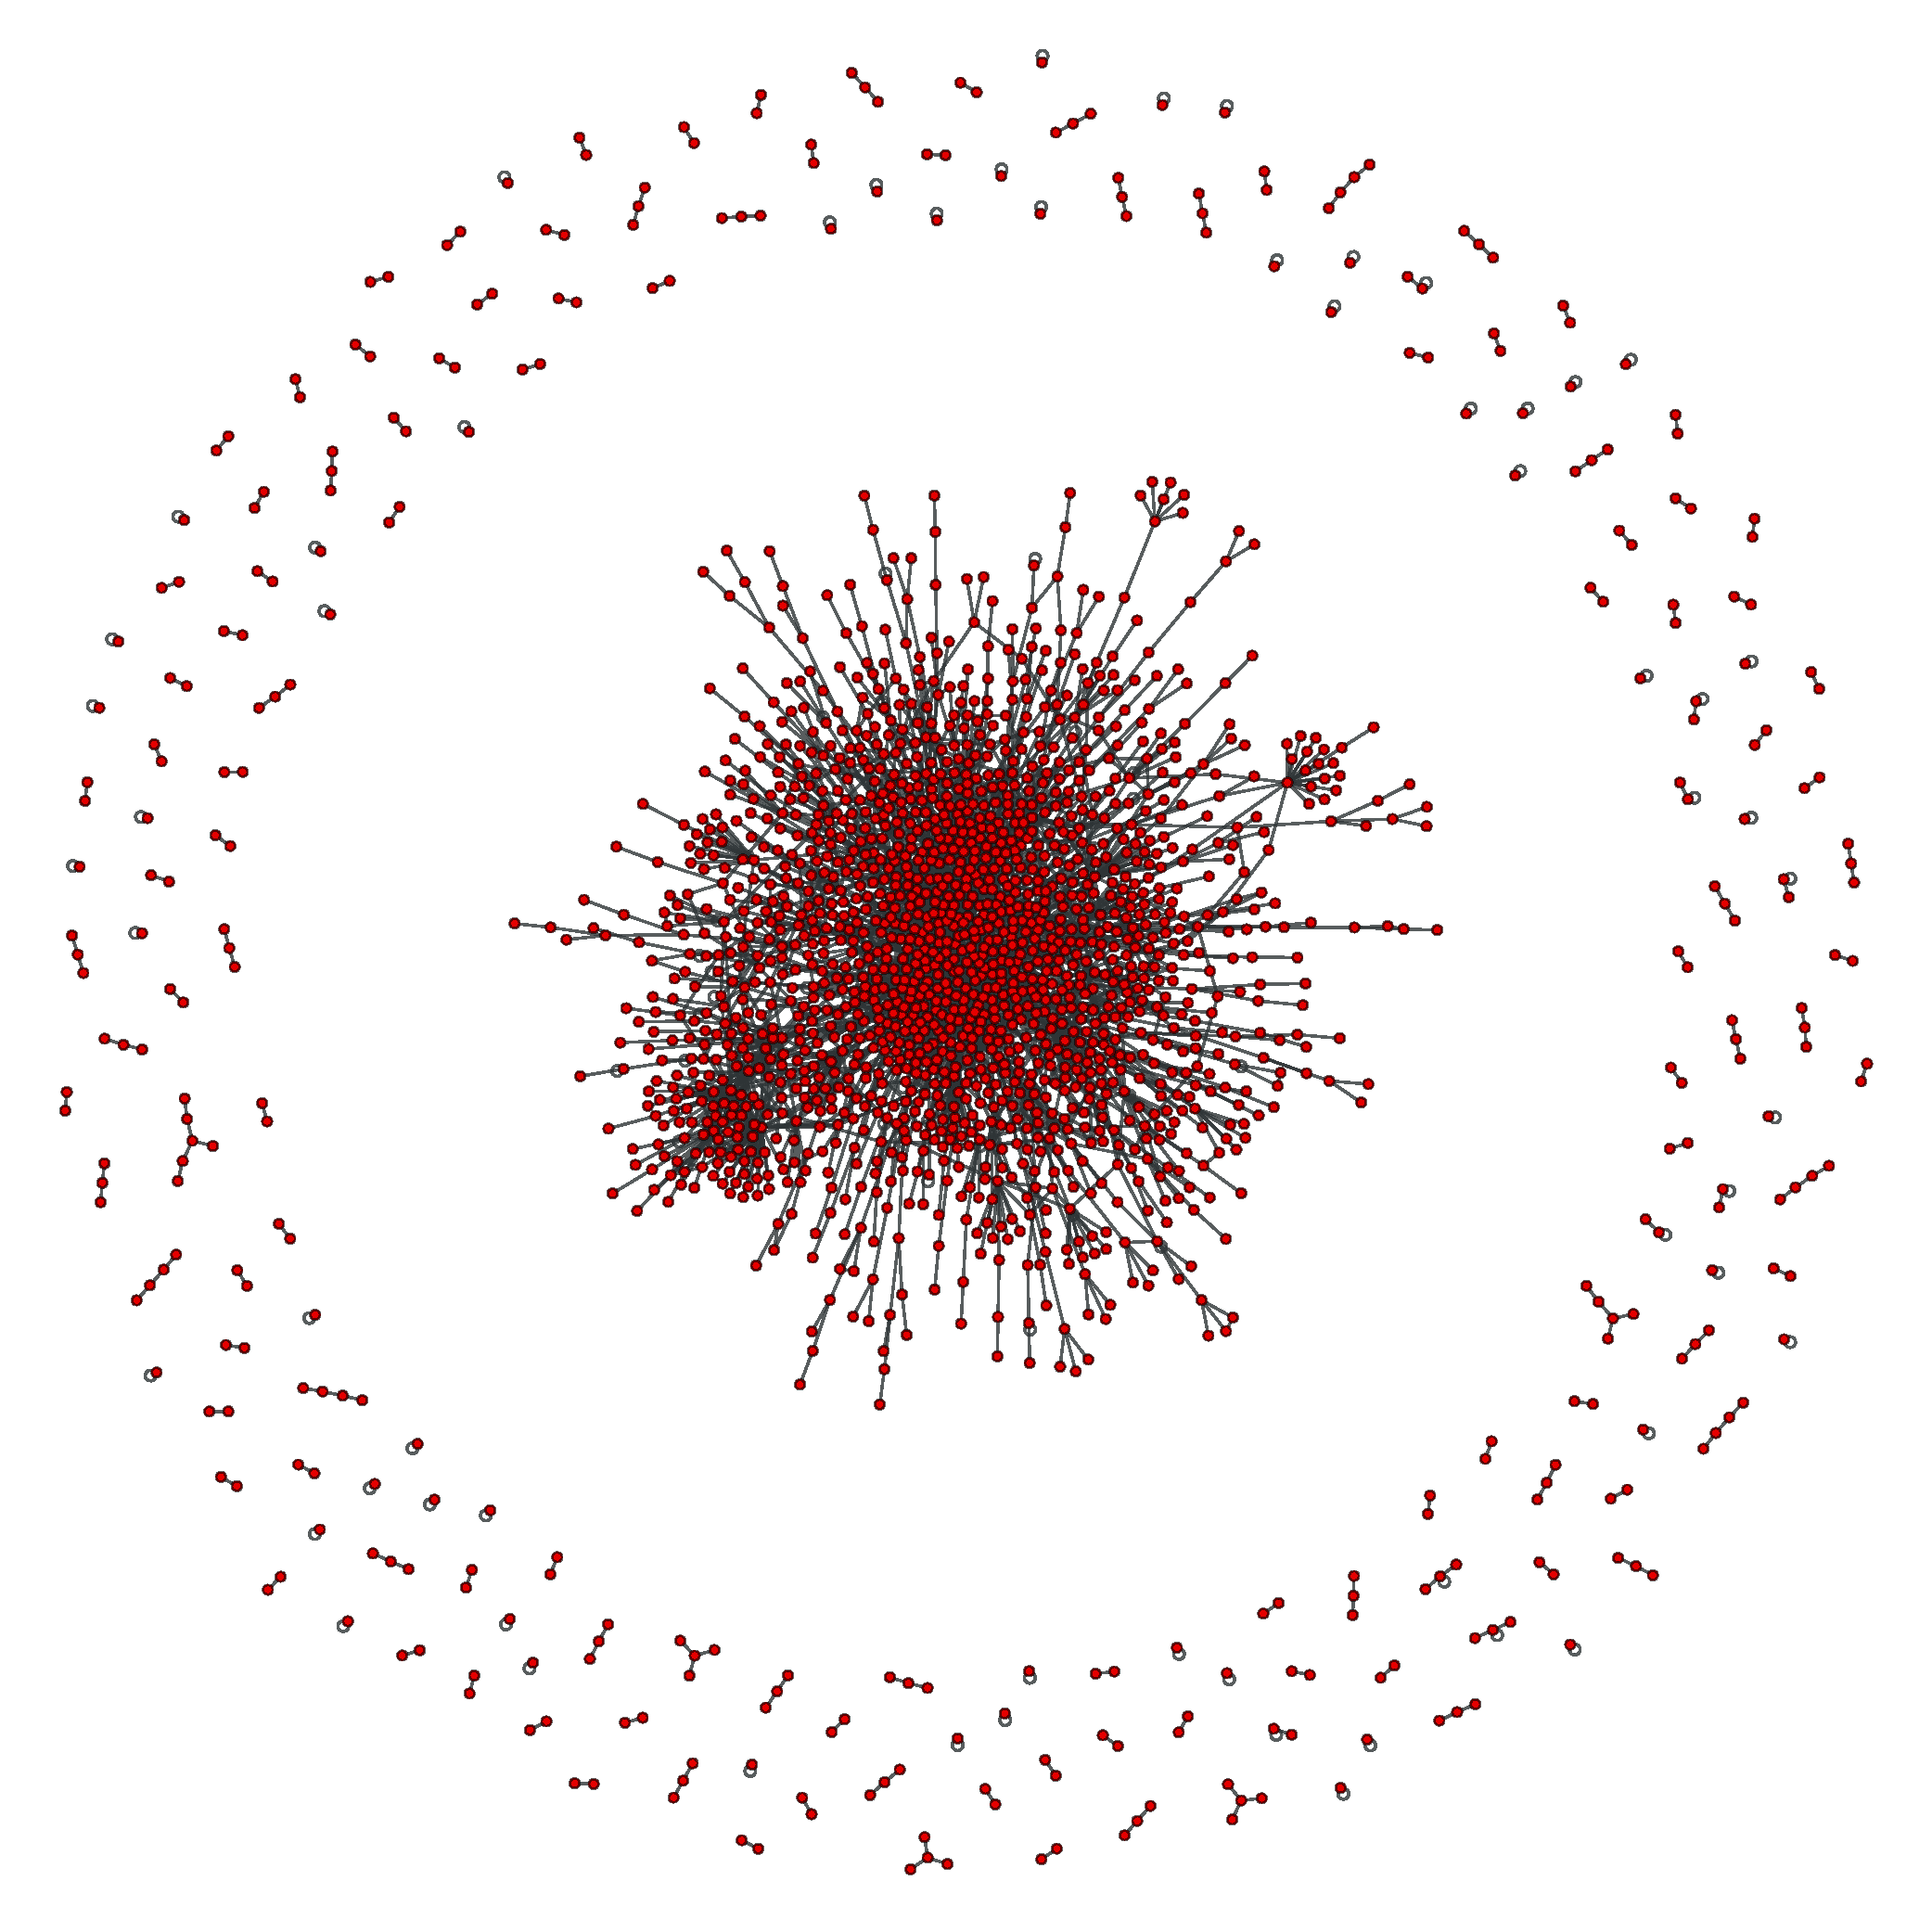
\includegraphics[width=\textwidth]{./schemes/yeast_Y2H-txt.pdf}
        \caption{\label{fig:y2h} Y2H}
    \end{subfigure}
    \\
    \begin{subfigure}[b]{0.4\columnwidth}
        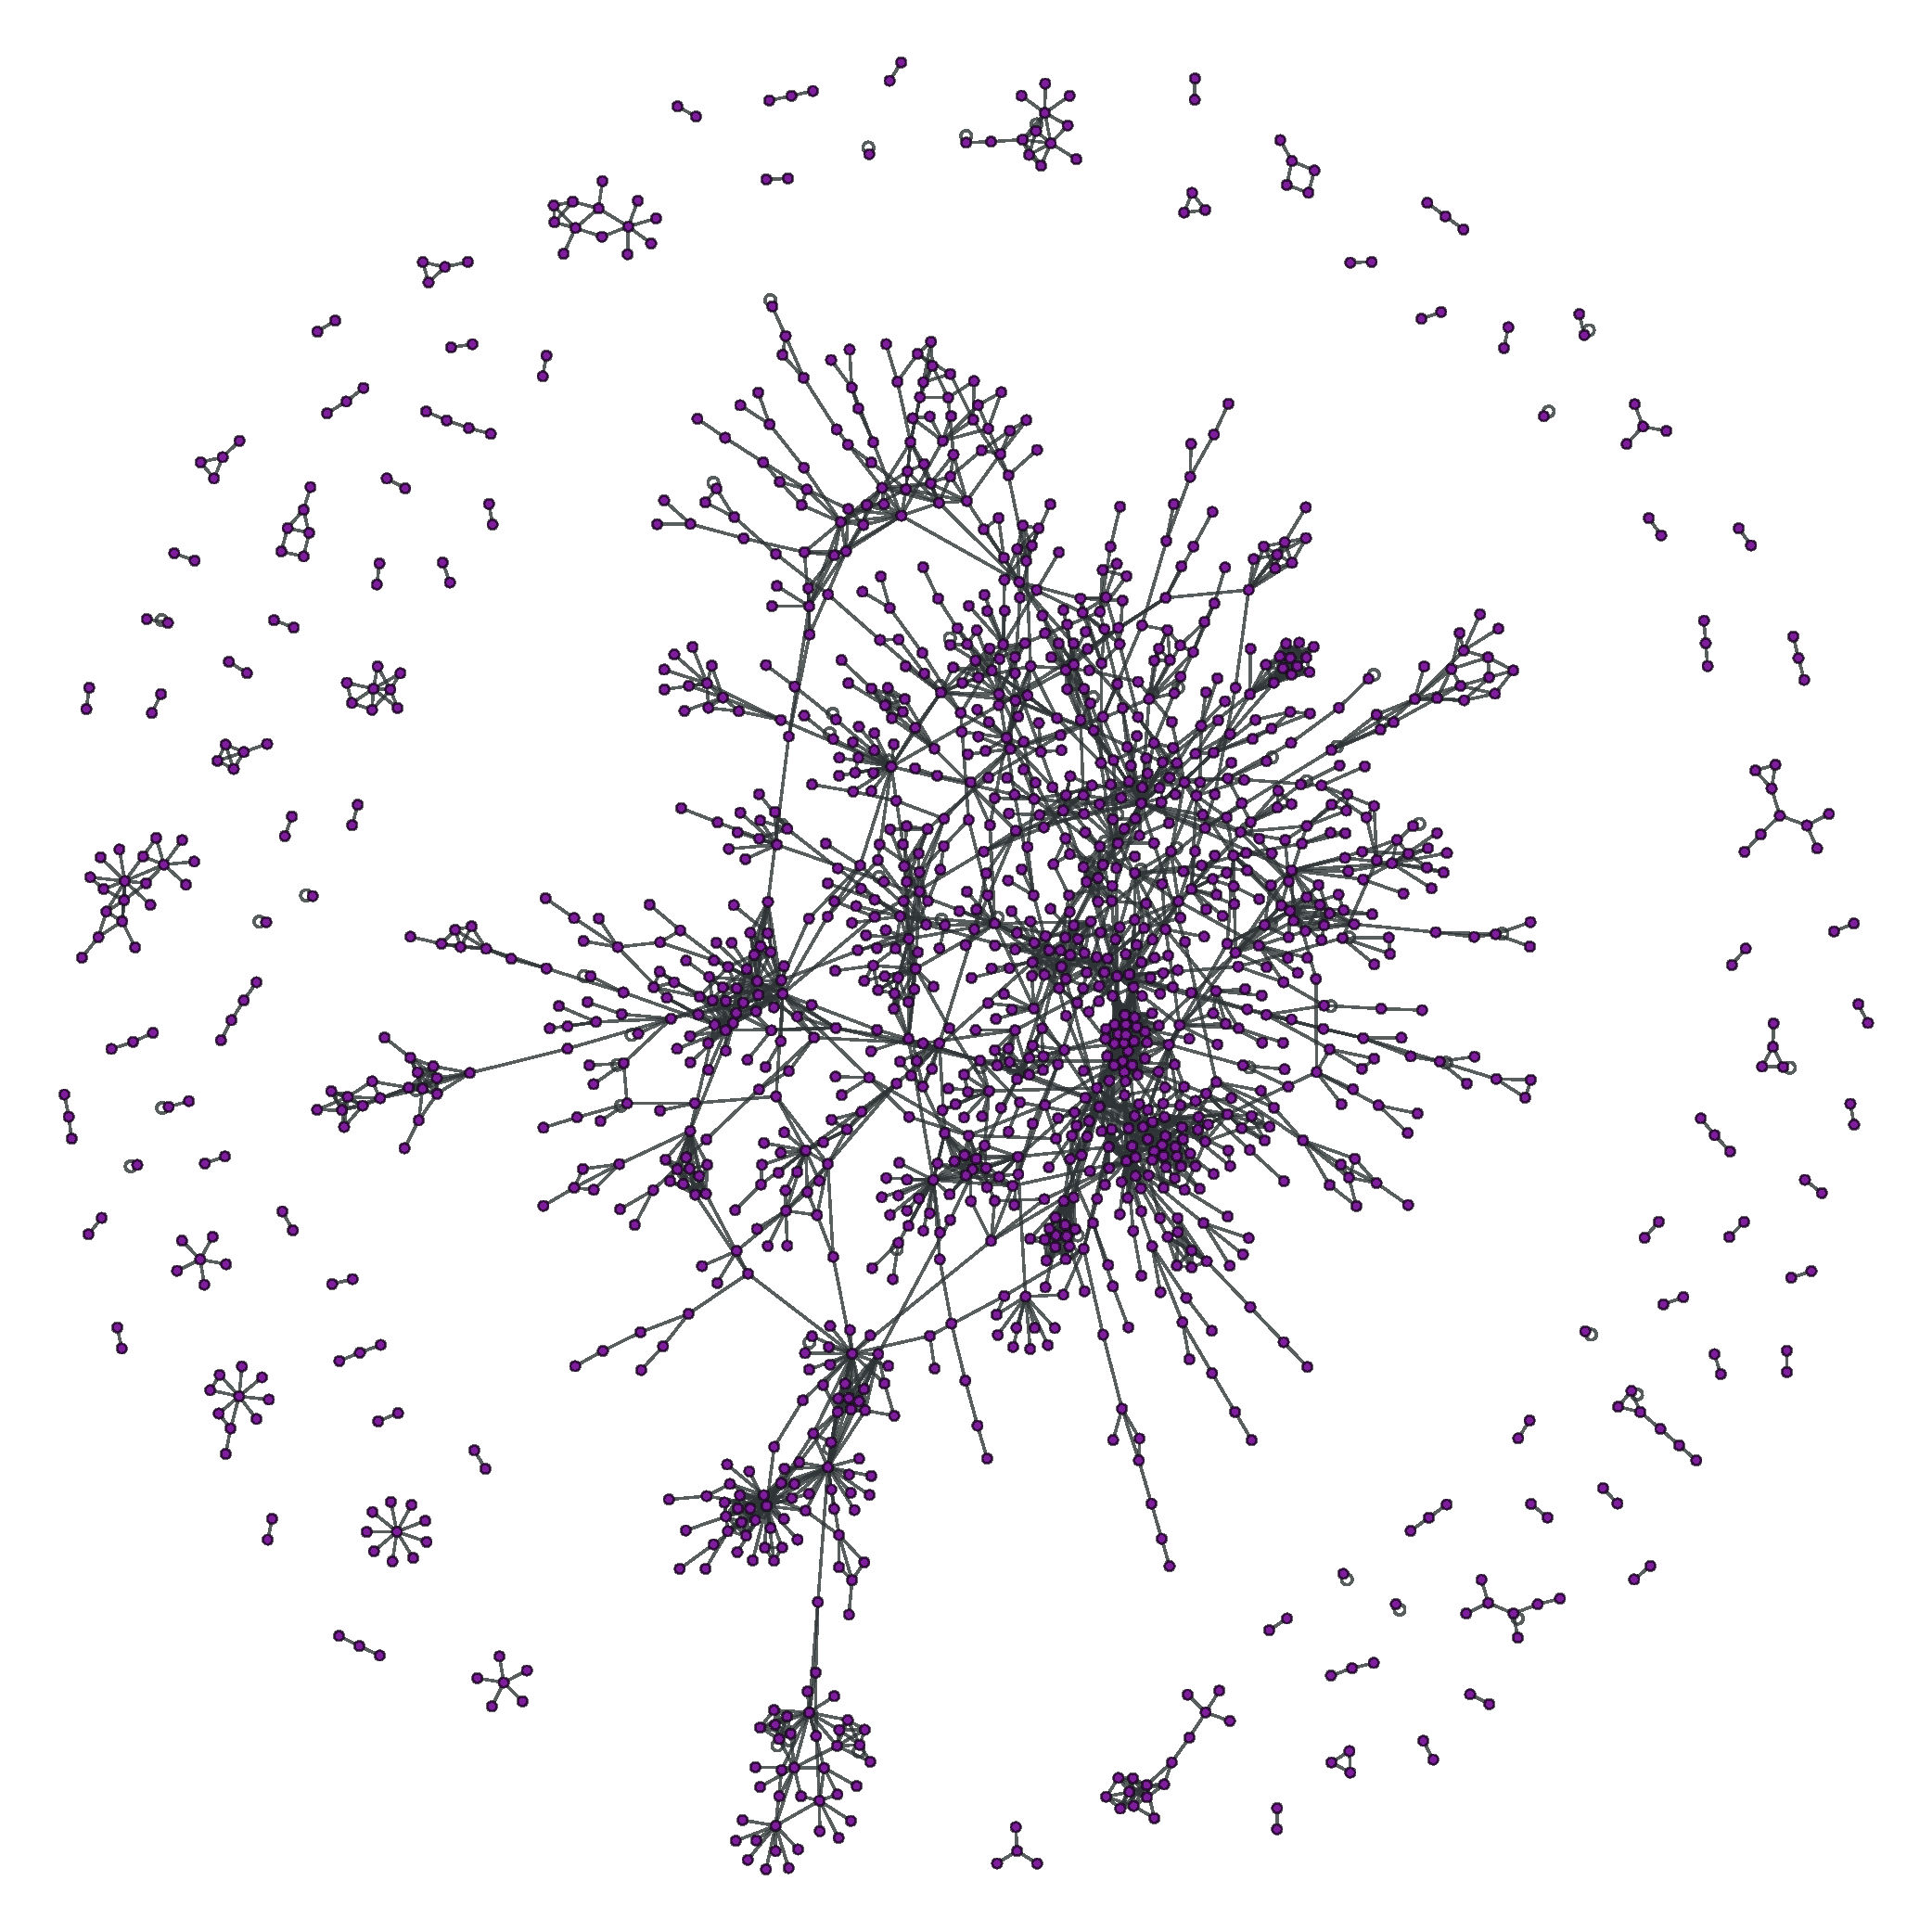
\includegraphics[width=\textwidth]{./schemes/yeast_LIT-txt.pdf}
        \caption{\label{fig:LIT}LIT}
    \end{subfigure}
    \begin{subfigure}[b]{0.4\columnwidth}
        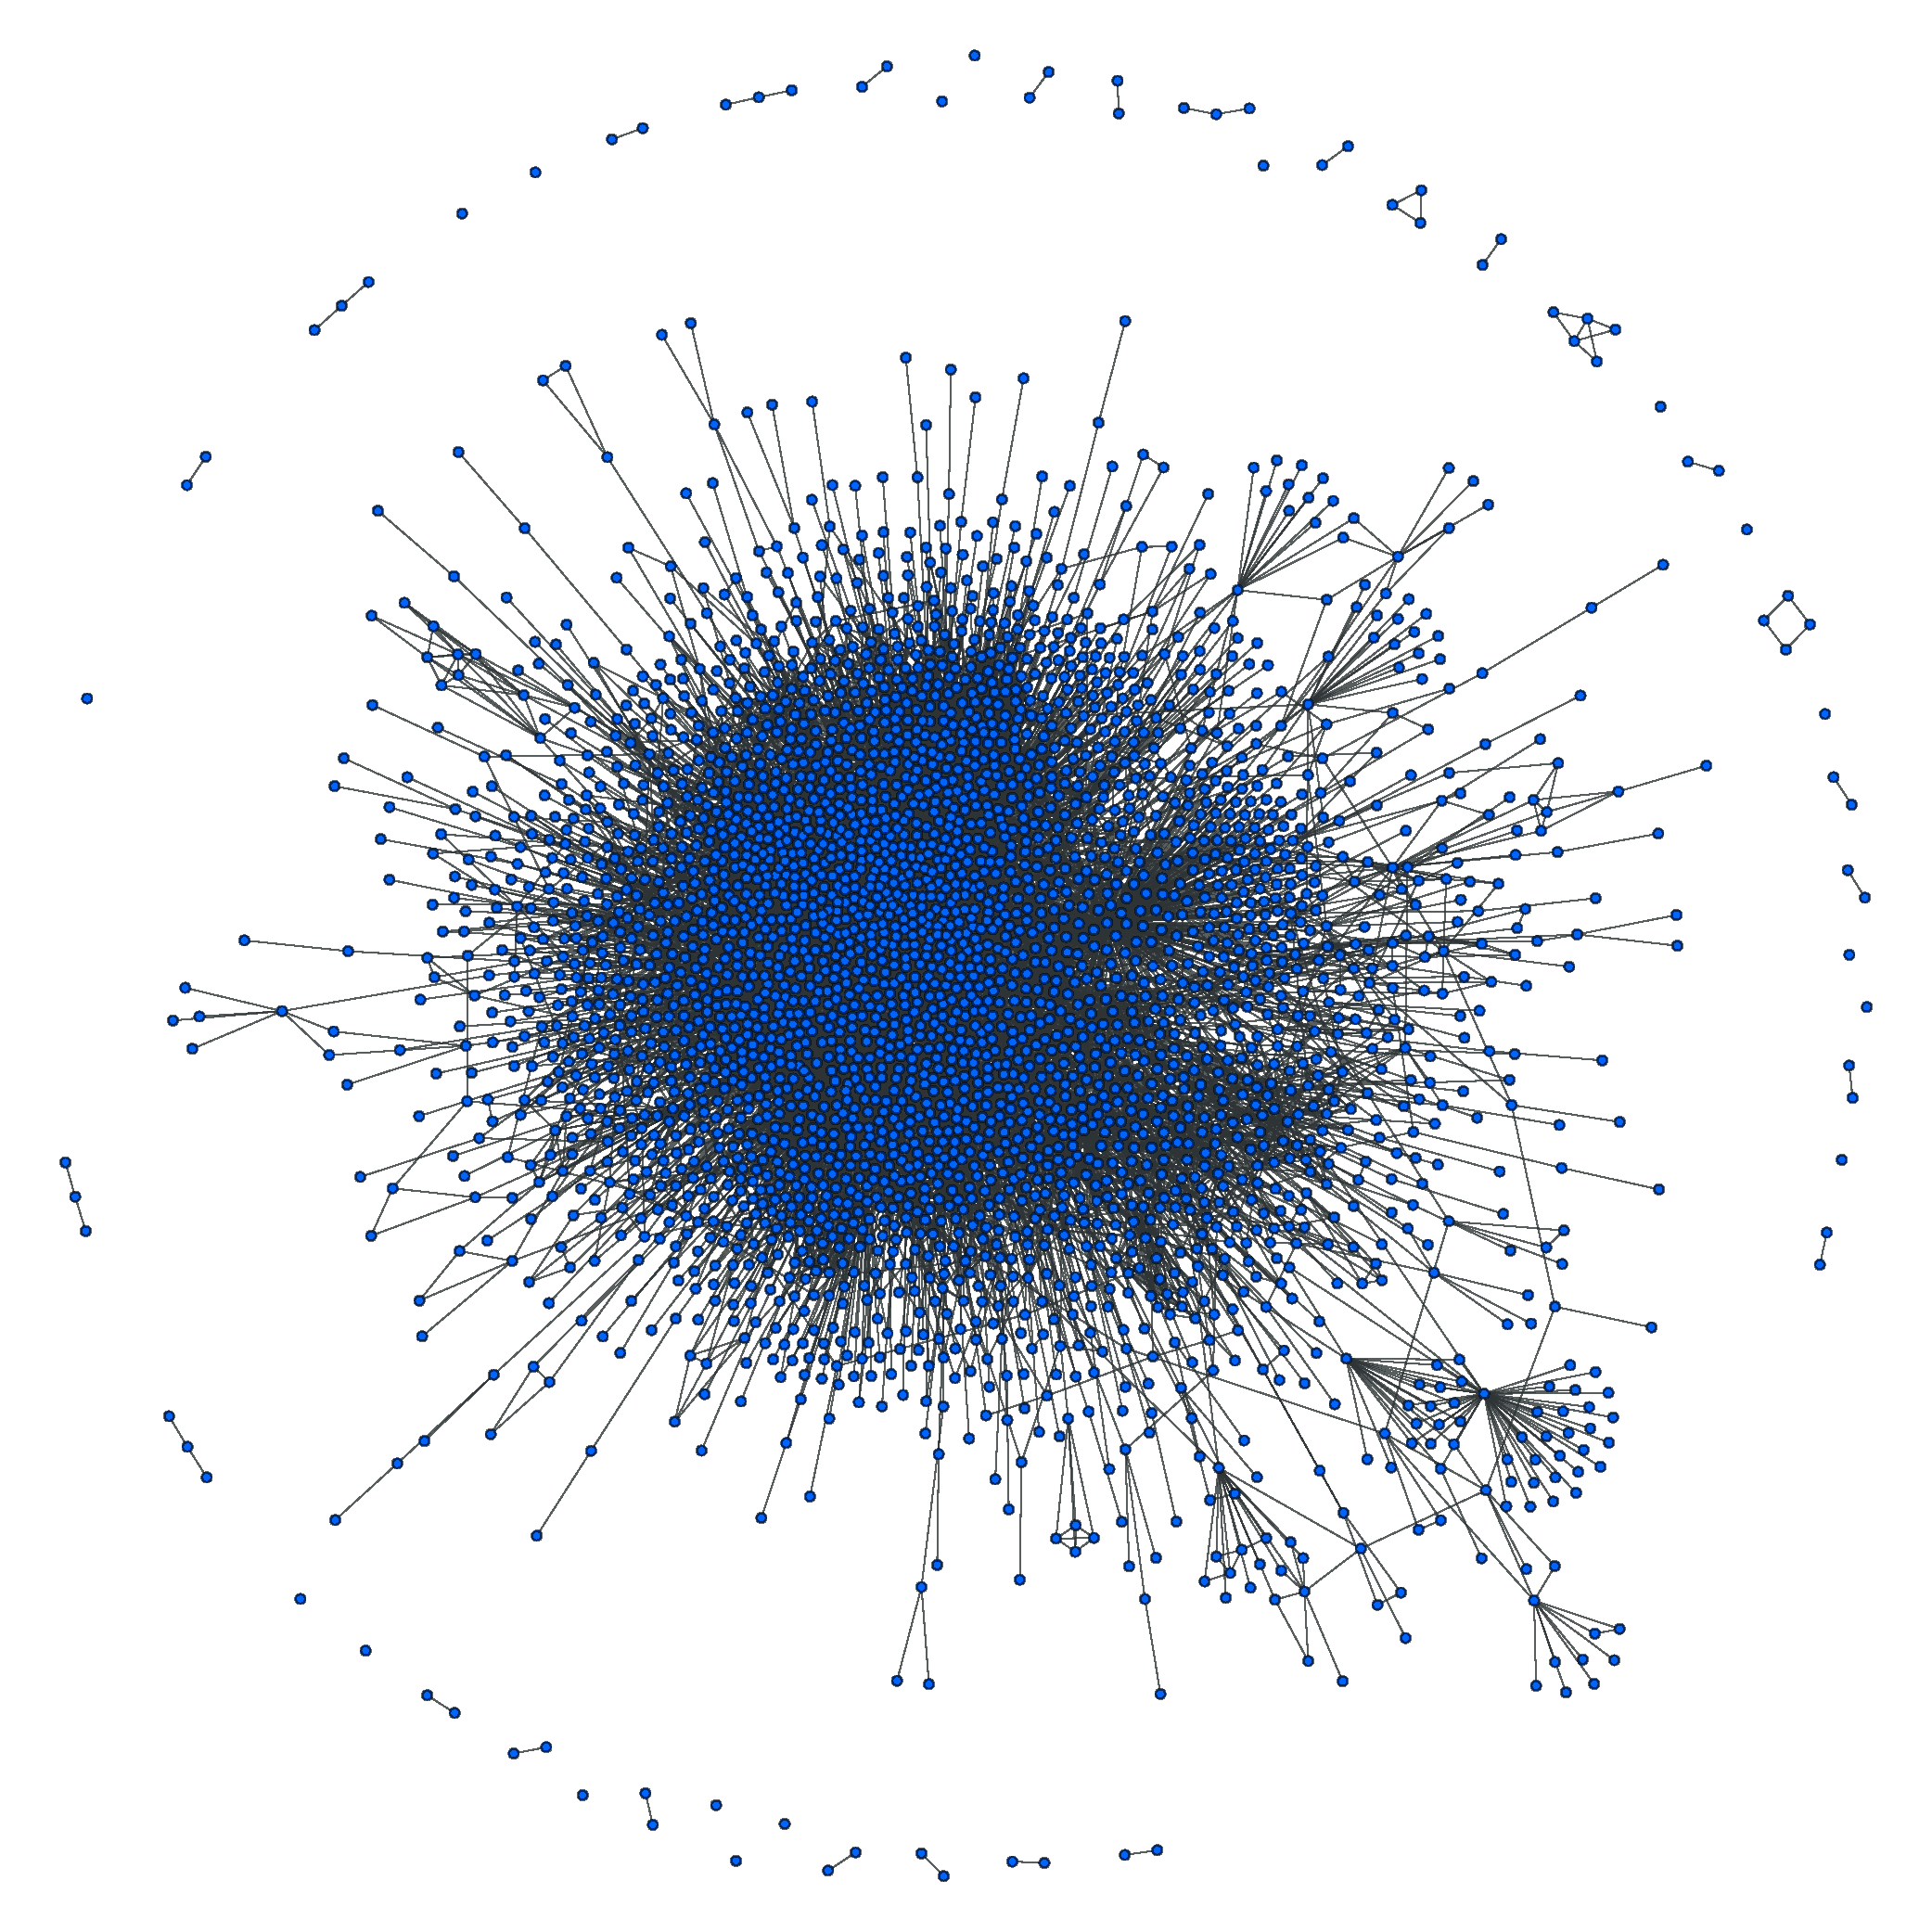
\includegraphics[width=\textwidth]{./schemes/yeast_LIT_Reguly-gml.pdf}
        \caption{\label{fig:LITR}LIT\_Reguly}
    \end{subfigure}
    \caption{\label{grafos} Esquematizaci\'on de los grafos de cada 
    red estudiada.}
\end{figure}

La tabla \ref{tab:obs} muestra un resumen de los observables estad\'isticos desprendidos de las propiedades topol\'ogicas de las redes. Por otro lado, la tabla \ref{tab:overlap} muestra la covertura entre cada par de redes. 

Es importante notar que debido a las diversas t\'ecnicas de construcci\'on de las redes, estas presentan diferencias significativas entre sus observables, como por ejemplo, no es extraño que la red AP-MS sea la que presenta mayor clusterizaci\'on y grado medio debido a que sus enlaces est\'an formados a partir de co-pertenencia a complejos proteicos, mientras que, por ejemplo, Y2H da cuenta de interacciones binarias/f\'isicas entre las proteinas. Adem\'as a partir de la tabla \ref{tab:overlap} se puede ver que las proteinas (nodos) en la red LIT, est\'an totalmente cubiertas por la red LIT\_Reguly, sin embargo esta \'ultima s\'olo cubre un 5\% de los enlaces de la red LIT.



\begin{table}[!ht]
    \centering
    \caption{\label{tab:obs}Observables para las cuatro redes de interacci\'on proteica de levadura.}
    {\scriptsize
    \begin{tabularx}{1\columnwidth}{XlX|XccccX}
        \hline\hline
        &\multirow{2}{*}{Observables}        &&& \multirow{2}{*}{AP-MS} & \multirow{2}{*}{LIT} & \multirow{2}{*}{Y2H} & \multirow{2}{*}{LIT\_Reguly} &\\ 
        &&&&&&\\
        \hline
        &N$^o$ nodos $N$    &&& 1622 & 1536 & 2018 &  3307 &\\
        &N$^o$ enlaces $L$  &&& 9070 & 2925 & 2930 & 11334 &\\
        &Densidad           &&& 0.0068 & 0.0024 & 0.0014 & 0.0020&\\
        &Diametro           &&& 15 & 19 & 14 & 12\\
        \hline
        &Grado $k$&&&\\
  %      \hline
        &\quad medio  $\mean{k}$     &&& 11.18 & 3.80& 2.93 & 6.85 &\\
        &\quad maximo $\max(\{k\})$  &&& 127  & 40   & 91 & 318&\\ 
        &\quad minimo $\min(\{k\})$  &&& 1    & 1    & 1 & 0&\\ 
        \hline
        &Coeficiente de Clusterizaci\'on&&&\\
        \hline
        &\quad medio/local $\mean{C}$               &&& 0.0710 & 0.4556 & 0.0970 & 0.3583&\\
        &\quad triangular/global $C_\bigtriangleup$ &&& 0.6185 & 0.3461 & 0.0236 & 0.1241&\\
        \hline\hline
    \end{tabularx}
    }
\end{table}

\begin{table}[!ht]
    \centering
    \caption{\label{tab:overlap}Observables para las tres redes de interacci\'on prote\'ica de levadura.}
    {\scriptsize
    \begin{tabularx}{.6\columnwidth}{XccccX}
        \hline\hline
        &AP-MS & 0.44 & 0.57 & 0.89 &\\
        &0.35& Y2H &0.36 & 0.66 &\\
        &0.60&0.48& LIT & 1.00 &\\
        &0.43&0.40& 0.46& LIT\_Reguly&\\
        \hline\hline
    \end{tabularx}
    }
\end{table}

%
%
%No es de extra\~nar que, a pesar de que estas 3 redes de proteinas 
%pertenecen al mismo organismo (\textit{Saccharomyces cerevisiae}),
%estas son distintas topol\'ogicamente debido a la manera en que son armadas.
%La red AP-MS muestra la formaci\'on de varios grupos/clusters muy densos que corresponden
%a los complejos proteicos purificados, esto se ve reflejado en los observables de la tabla \ref{tab:obs}
%en que, salvo el di\'ametro, presenta mayores valores que el resto de las redes. 
%Cabe observar que la red de literatura LIT presenta el mayor di\'ametro, sin embargo es la con 
%menor grado m\'aximo (por lo que pareciera capaz de relacionar m\'as interacciones entre clusters), debido a la compilaci\'on
%de un gran n\'umero de trabajos, pero tiene menor detalle de las interacciones prote\'ina-prote\'ina, debido
%a que en general los trabajos consultados son espec\'ificos y por lo tanto sesgados (hay perdida de informaci\'on las proteinas
%menos estudiadas).
%En particular al observar la clusterizaci\'on es importante diferenciar la clusterizaci\'on media $\mean{C}$ y la 
%clusterizaci\'on triangular $C_\bigtriangleup$. La primera caracteriza la media de la clusterizaci\'on local de cada 
%nodo, es por ello que la red LIT prensenta el mayor valor, debido a que, como mencionamos antes, compila
%trabajos detallados que dan cuenta de peque\~nos clusters. Tanto la red AP-MS y, a\'un m\'as, la red Y2H diluyen
%su clusterizaci\'on debido a un gran n\'umero de \textit{peque\~nas interacciones aisladas}. Por otro lado
%el coeficiente $C_\bigtriangleup$ es una medida m\'as global, ya que no pesa interacciones bin\'arias puras.
%En este \'ultimo caso AP-MS presenta la mayor clusterizaci\'on, mientras que Y2H la menor.
%
%
%\subsection{Coherencia entre las redes}
%
%\begin{figure}[!ht]
%    \centering
%    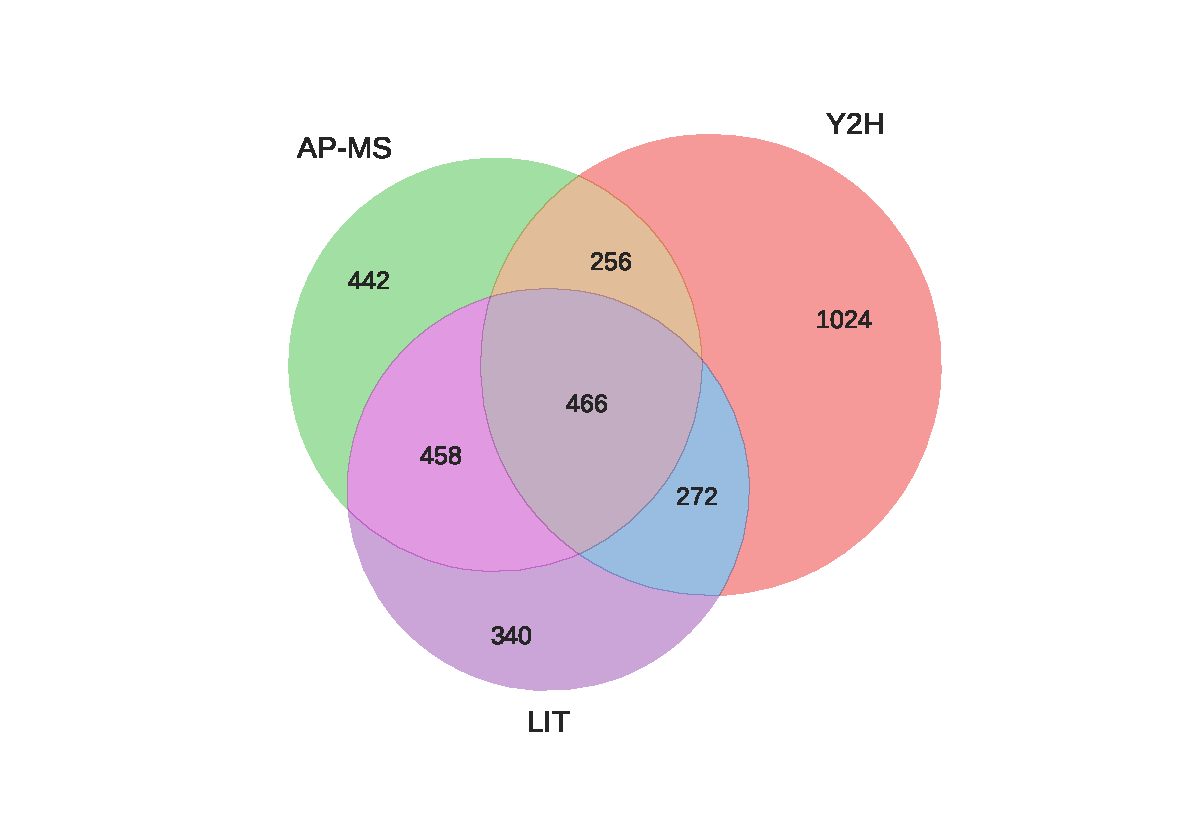
\includegraphics[width=.5\columnwidth]{./schemes/venn_AP-MS-Y2H-LIT_covertura.pdf}
%    \caption{\label{fig:cober} Diagrama de Venn para cobertura entre las tres redes. }
%\end{figure}
%
%
%
%En segundo lugar se analiz\'o la cobertura y coherencia entre las interacci\'ones reportadas
%en las redes. Para ello se realiz\'aron los diagramas de Venn mostrados en la figura \ref{fig:cober}, \ref{fig:venn} y \ref{fig:subgrafos}
%(estos pueden reproducirse con el script \texttt{venn.py} \texttt{venn2.py}). Para analizar la covertura comparamos
%la intersecci\'on de las prote\'inas reportadas en cada caso. En la figura \ref{fig:cober} se muestra
%la cobertura de cada red y la cantidad de proteinas reportadas por m\'as de una red (intersecciones). Es 
%interesante notar que AP-MS y LIT presentan $\sim 60\%$ de cobertura entre ellas y solo un $\sim 27\%$ 
%y un $\sim 22\%$ de las prot\'inas reportadas, respectivamente, son especificas de cada red. Esto se ve contrastado
%con el $\sim 50\%$ de especificidad en la red Y2H. 
%
%
%\vspace{1.5cm}
%\begin{figure}[!ht]
%    \centering
%    \begin{subfigure}[b]{0.48\columnwidth}
%        \centering
%        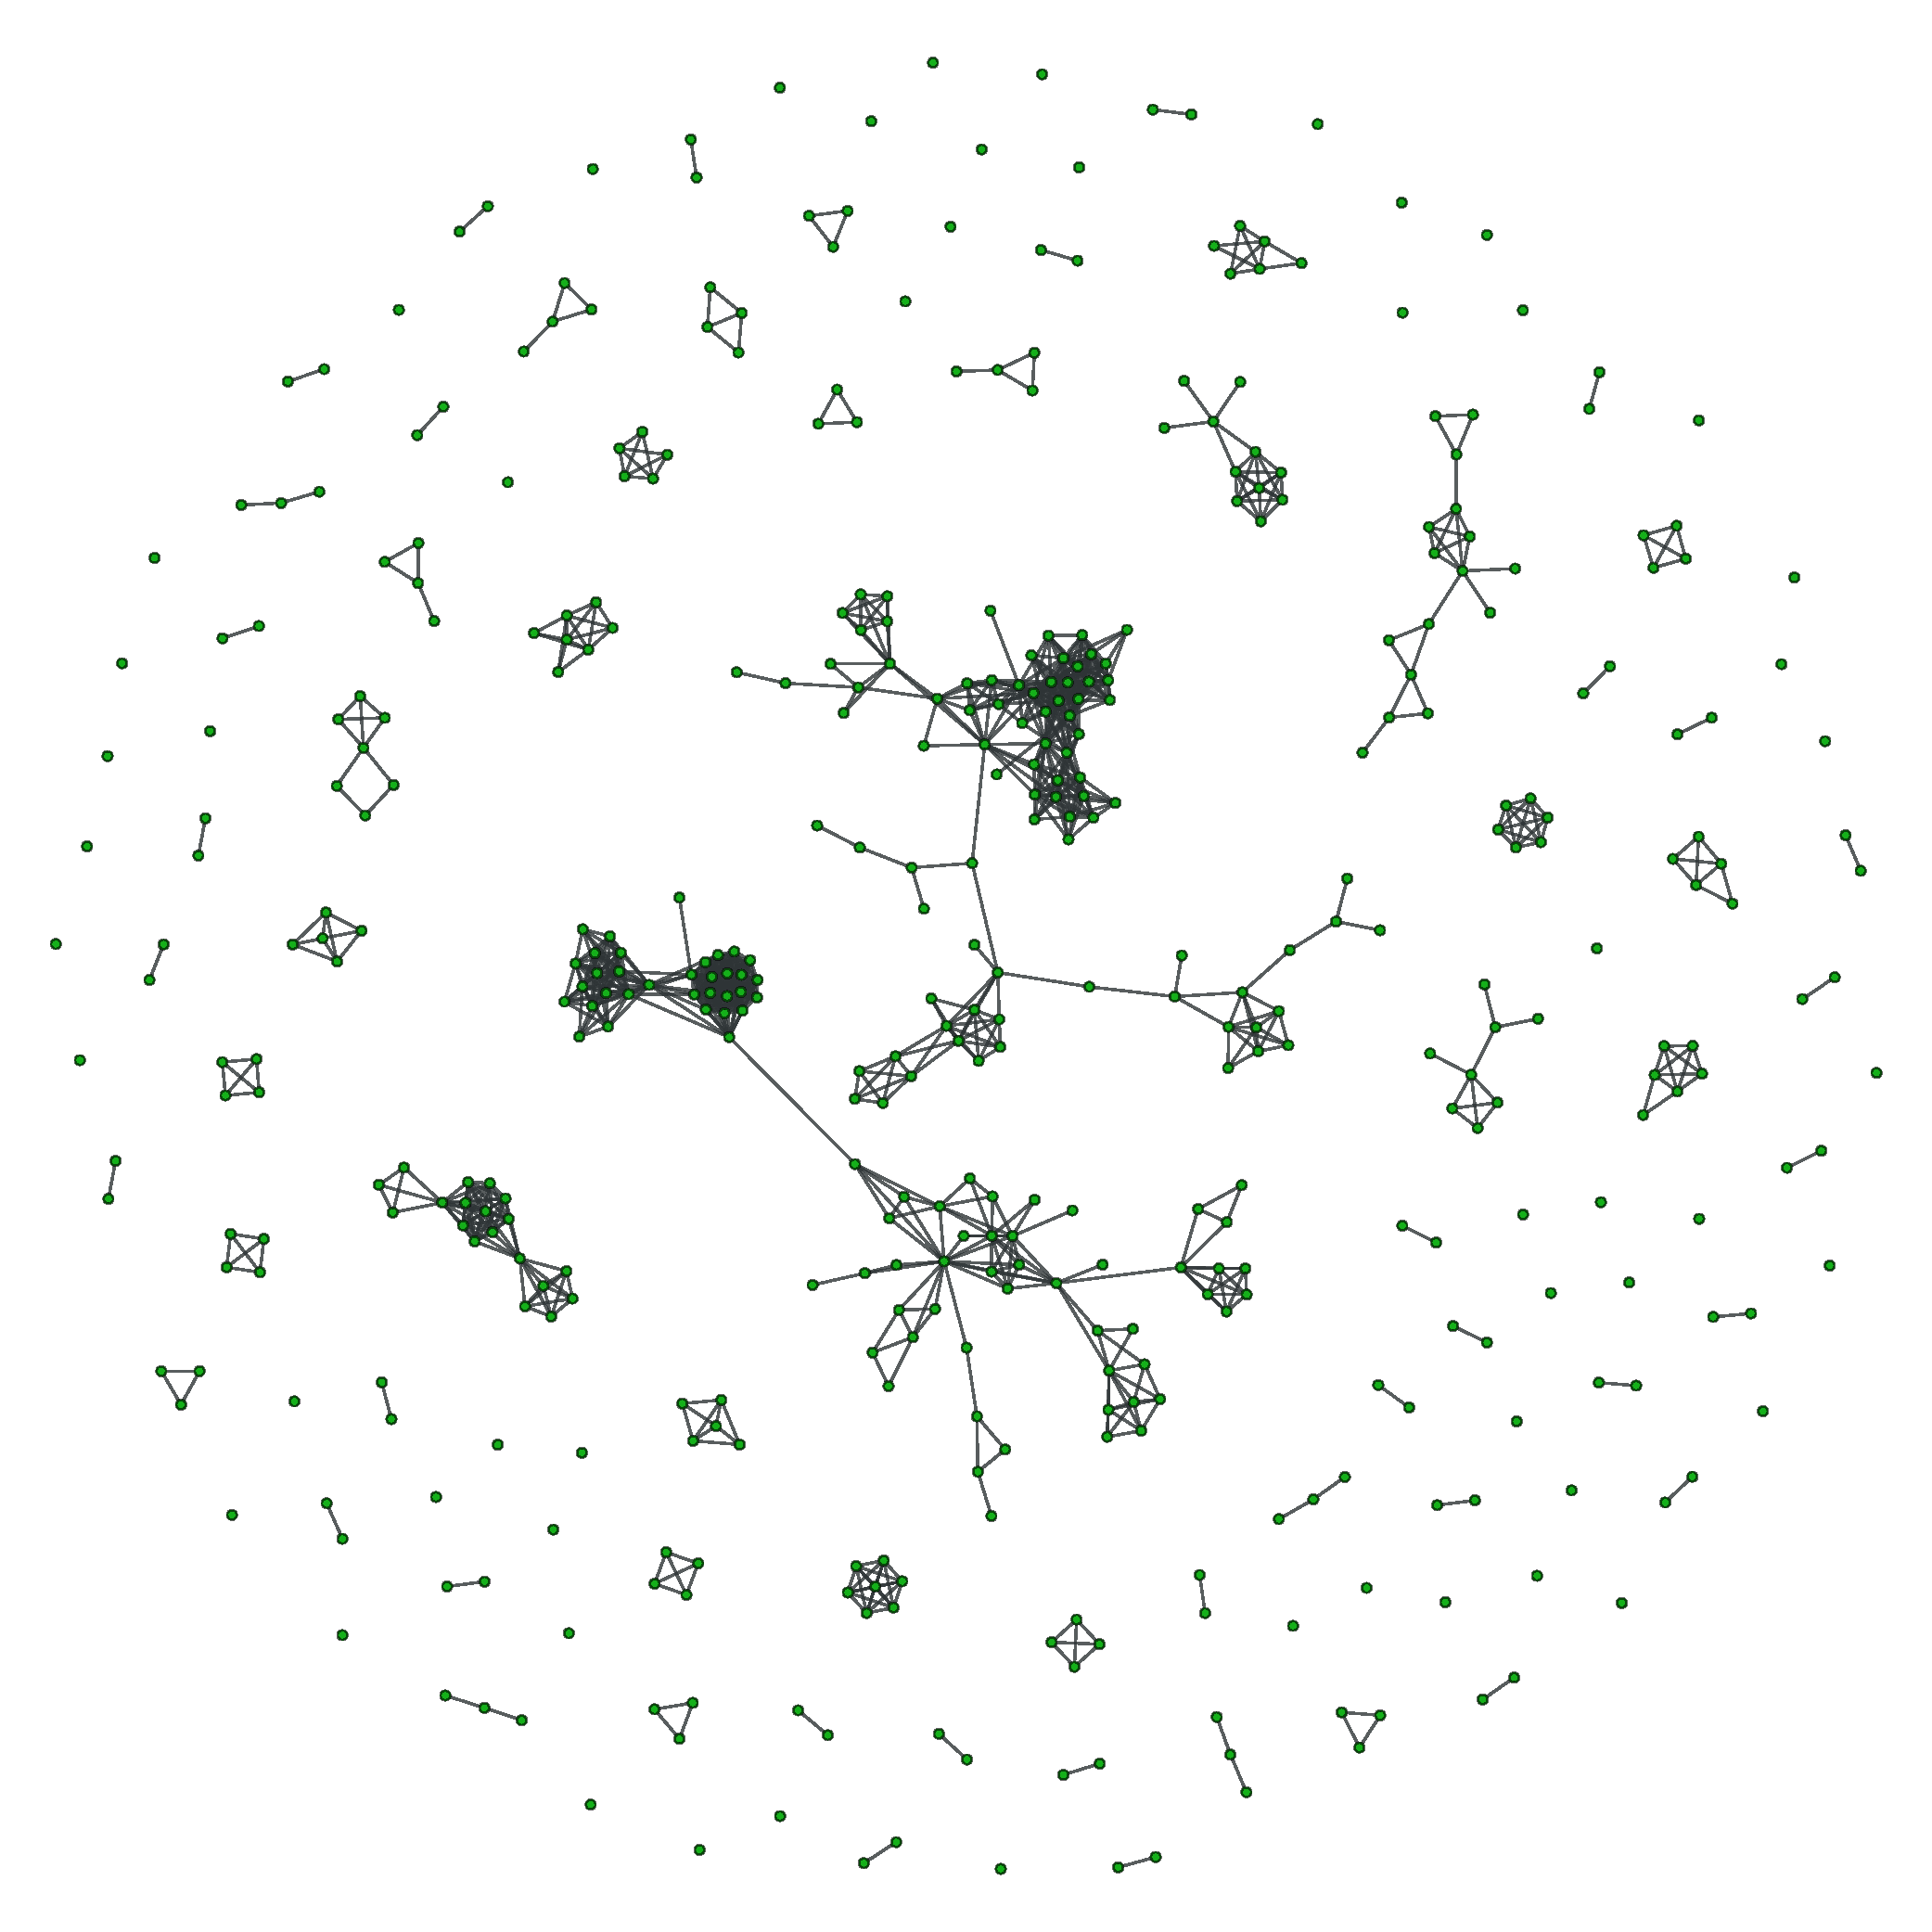
\includegraphics[width=.45\textwidth]{./schemes/subgrafo_AP-MS_all-gml.pdf}
%        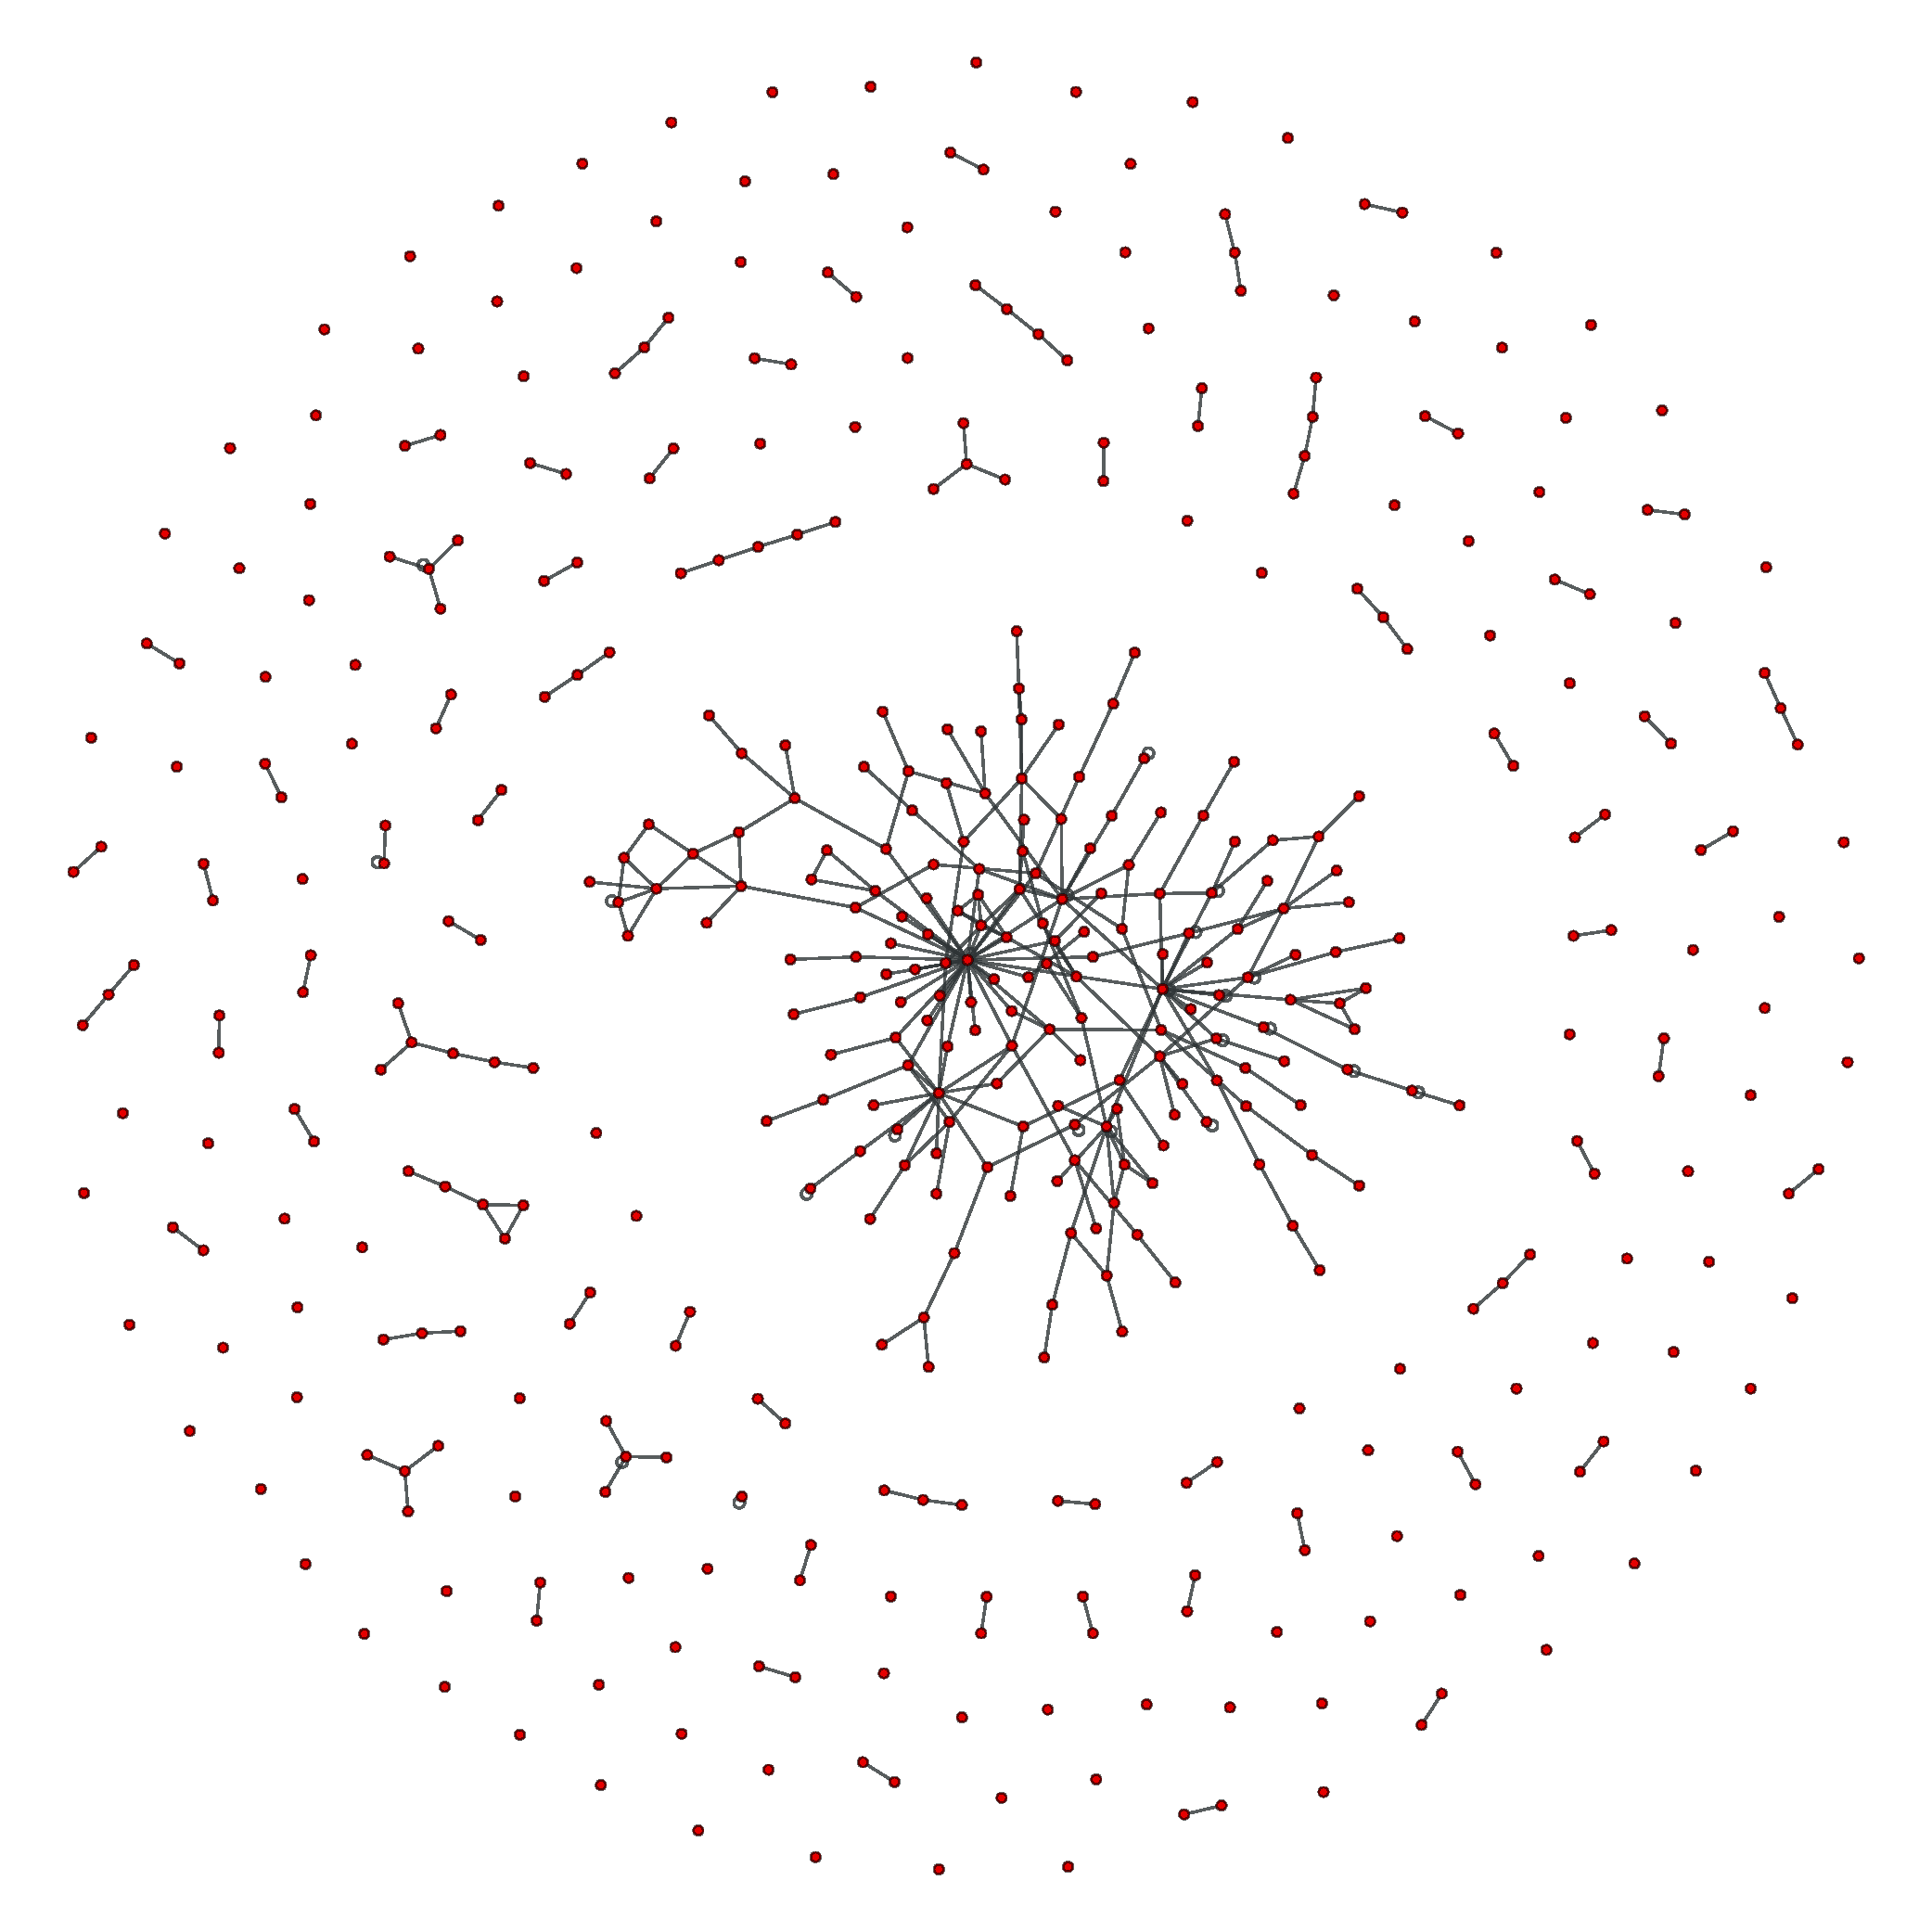
\includegraphics[width=.45\textwidth]{./schemes/subgrafo_Y2H_all-gml.pdf}\\
%        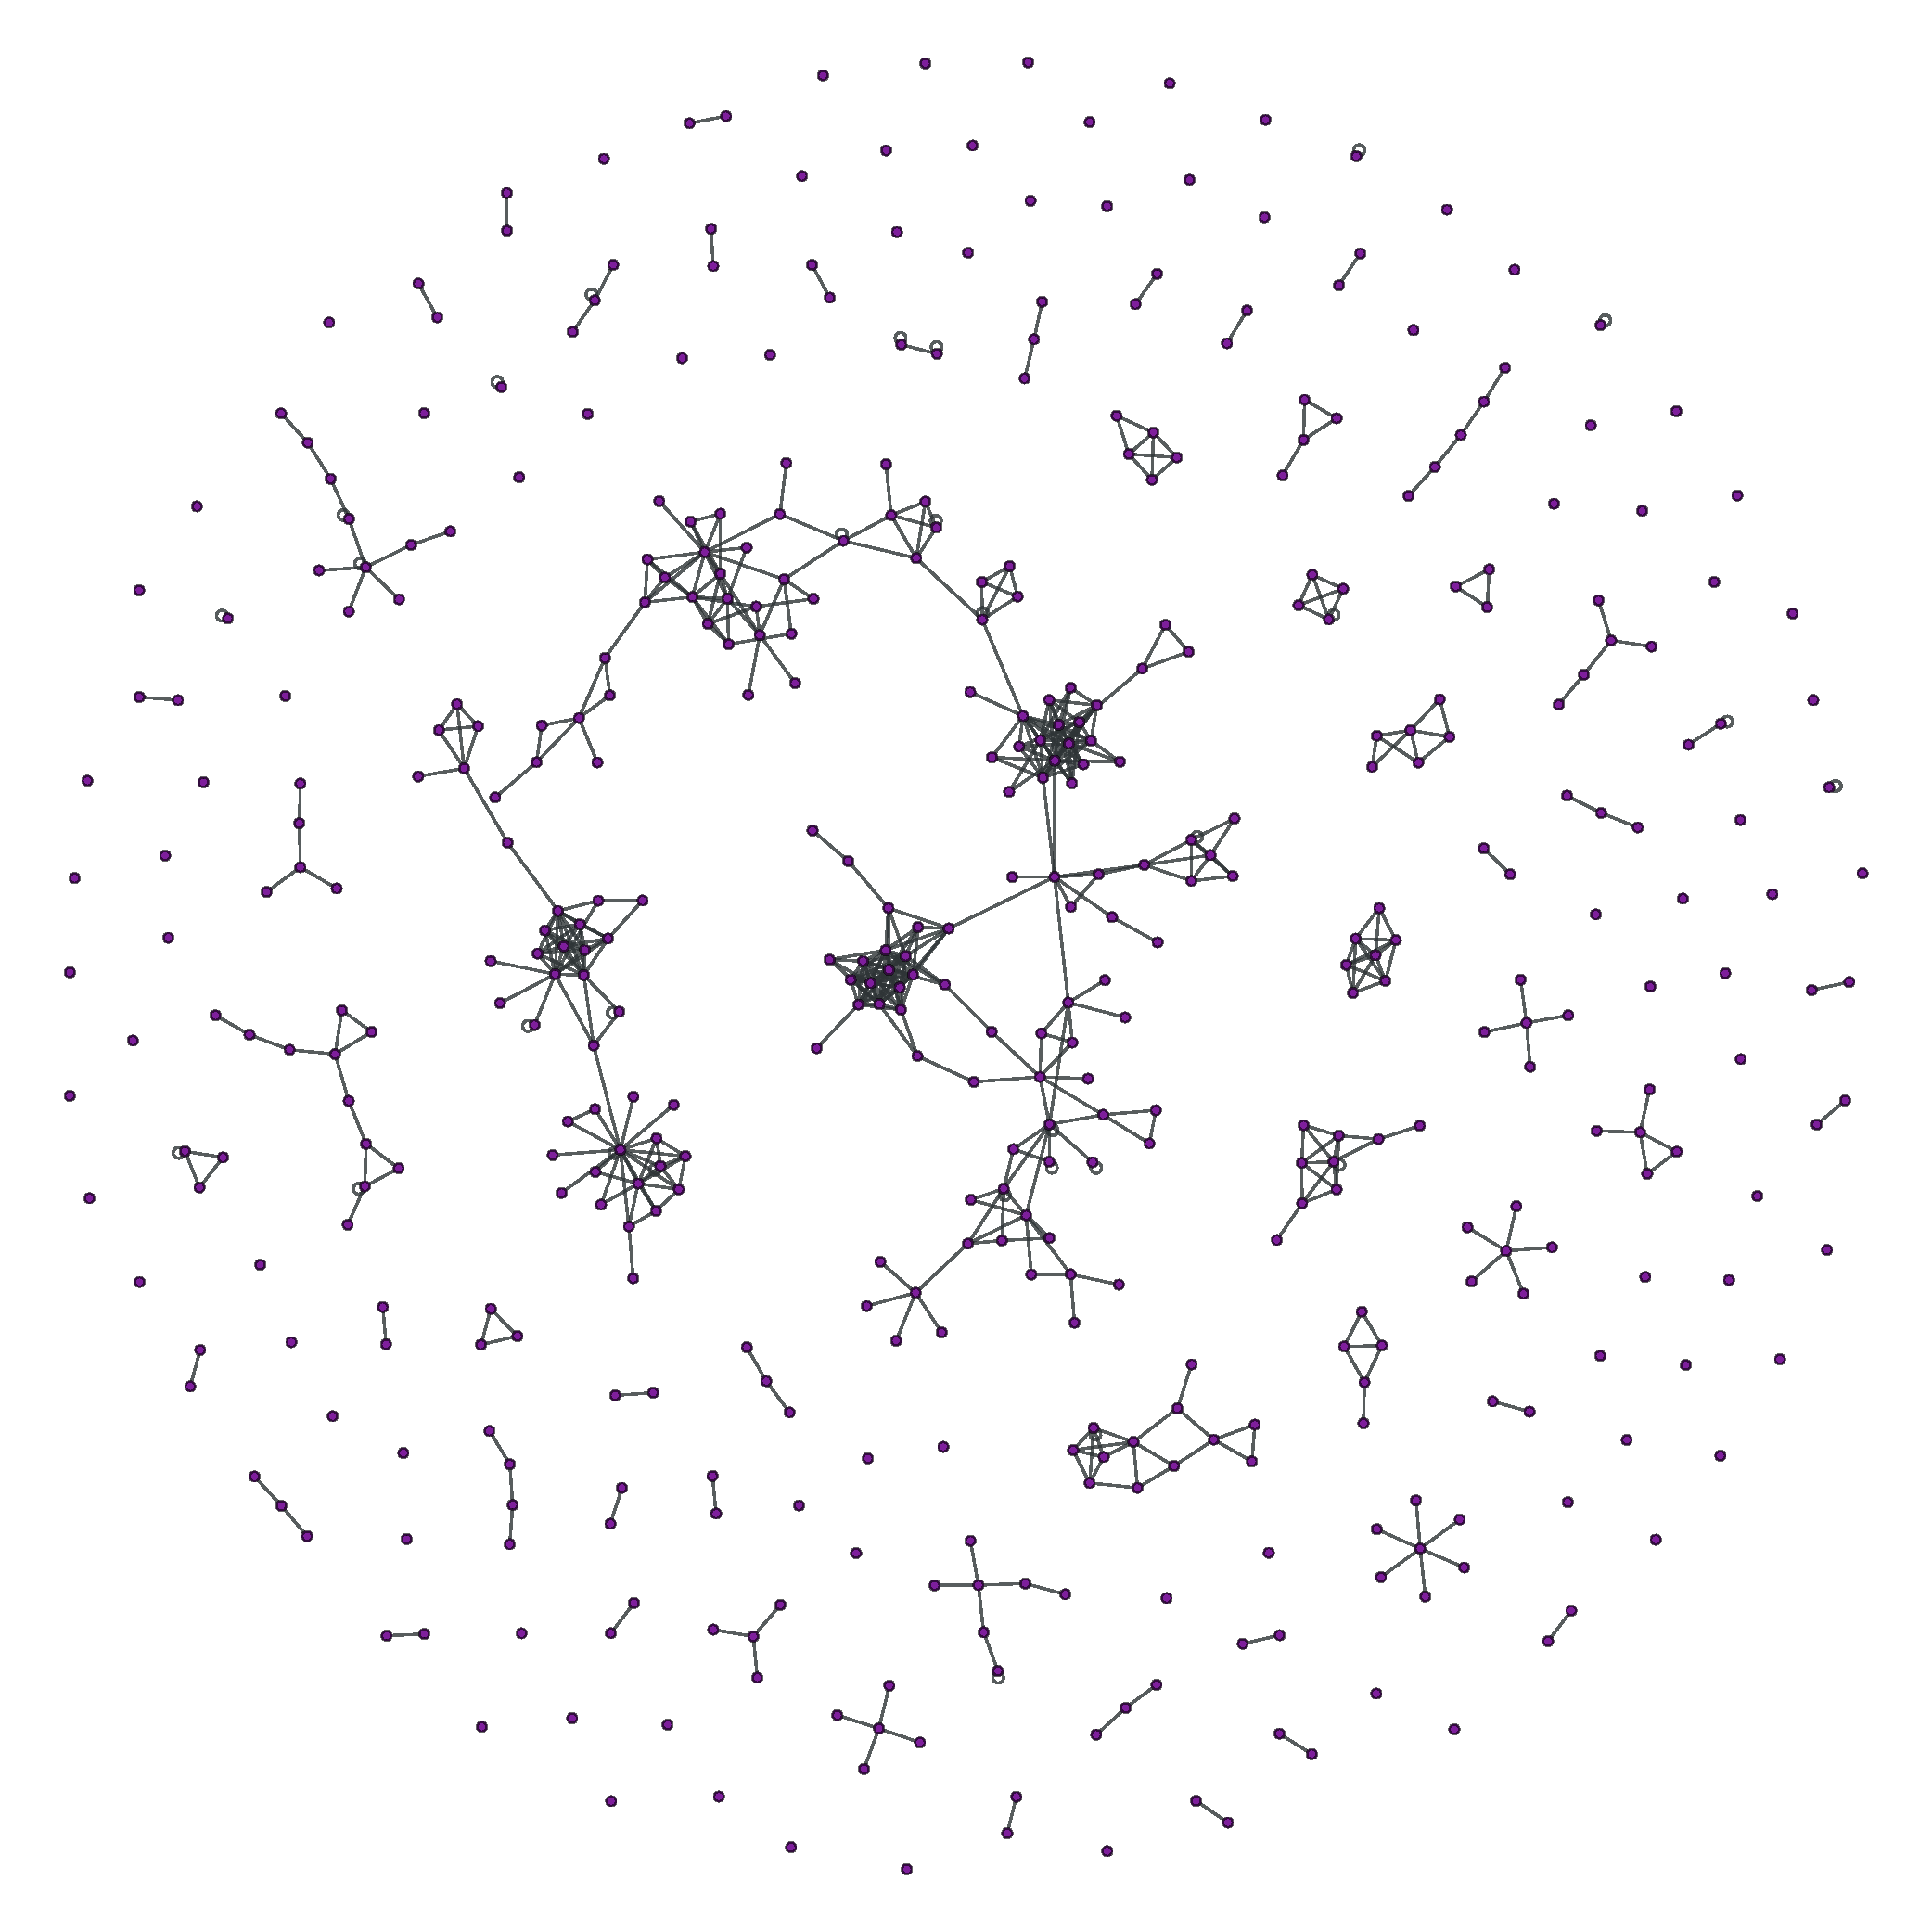
\includegraphics[width=.45\textwidth]{./schemes/subgrafo_LIT_all-gml.pdf}
%        \caption{\label{fig:all} AP-MS/Y2H/LIT}
%    \end{subfigure}
%    \hfill
%    \begin{subfigure}[b]{0.48\columnwidth}
%        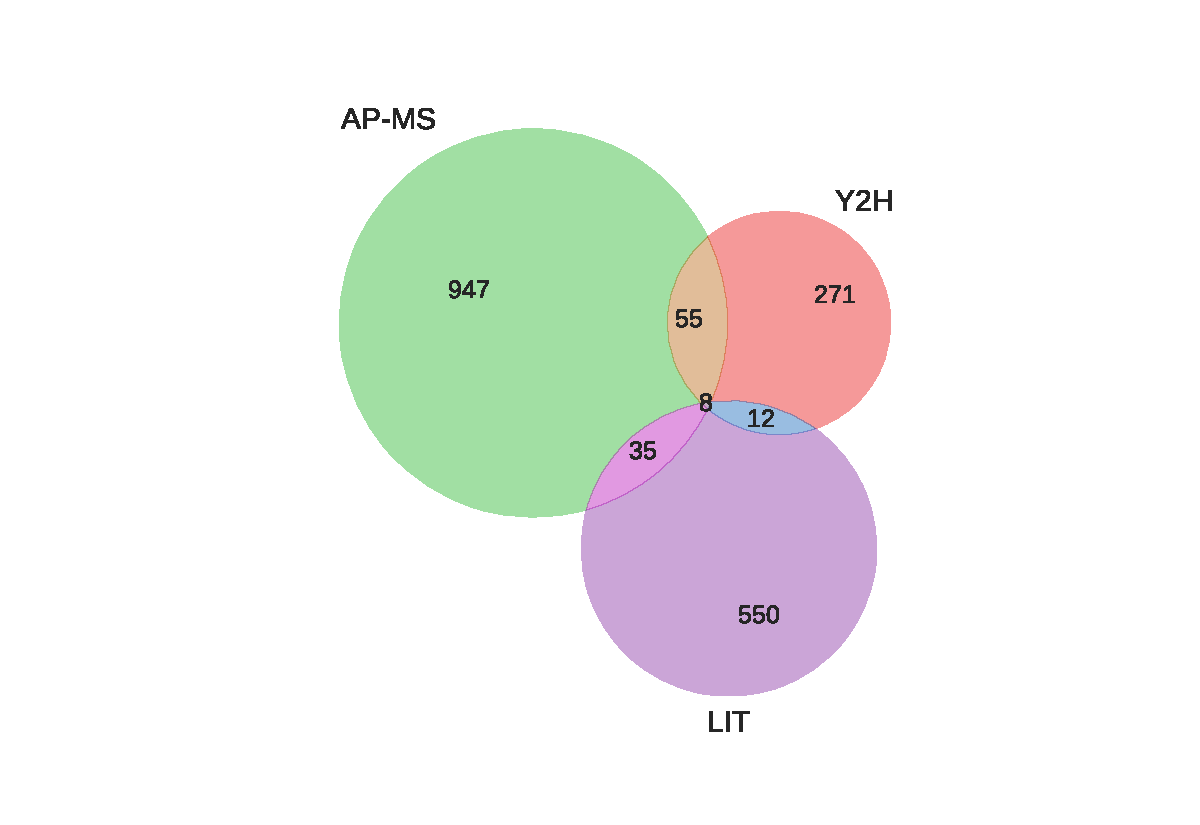
\includegraphics[width=\textwidth]{./schemes/venn_AP-MS-Y2H-LIT_links.pdf}
%        \caption{\label{fig:cohe} Coherencia}
%    \end{subfigure}
%    \caption{\label{fig:venn} Subgrafos inducidos por cobertura de las 3 redes y coherencia de links entre ellas. }
%\end{figure}
%
%\vspace{1.5cm}
%Por otra parte, a partir de la intersecci\'on de las prote\'inas reportadas de las tres redes, se analiza la coherencia
%de los enlaces entre las prote\'inas comunes. De la figura \ref{fig:cohe} se puede observar al alta especificidad
%de cada red respecto al resto (solo 8 links son compartidos por las tres redes). 
%
%
%\begin{figure}[!ht]
%    \centering
%    \begin{subfigure}[b]{0.3\columnwidth}
%        \centering
%        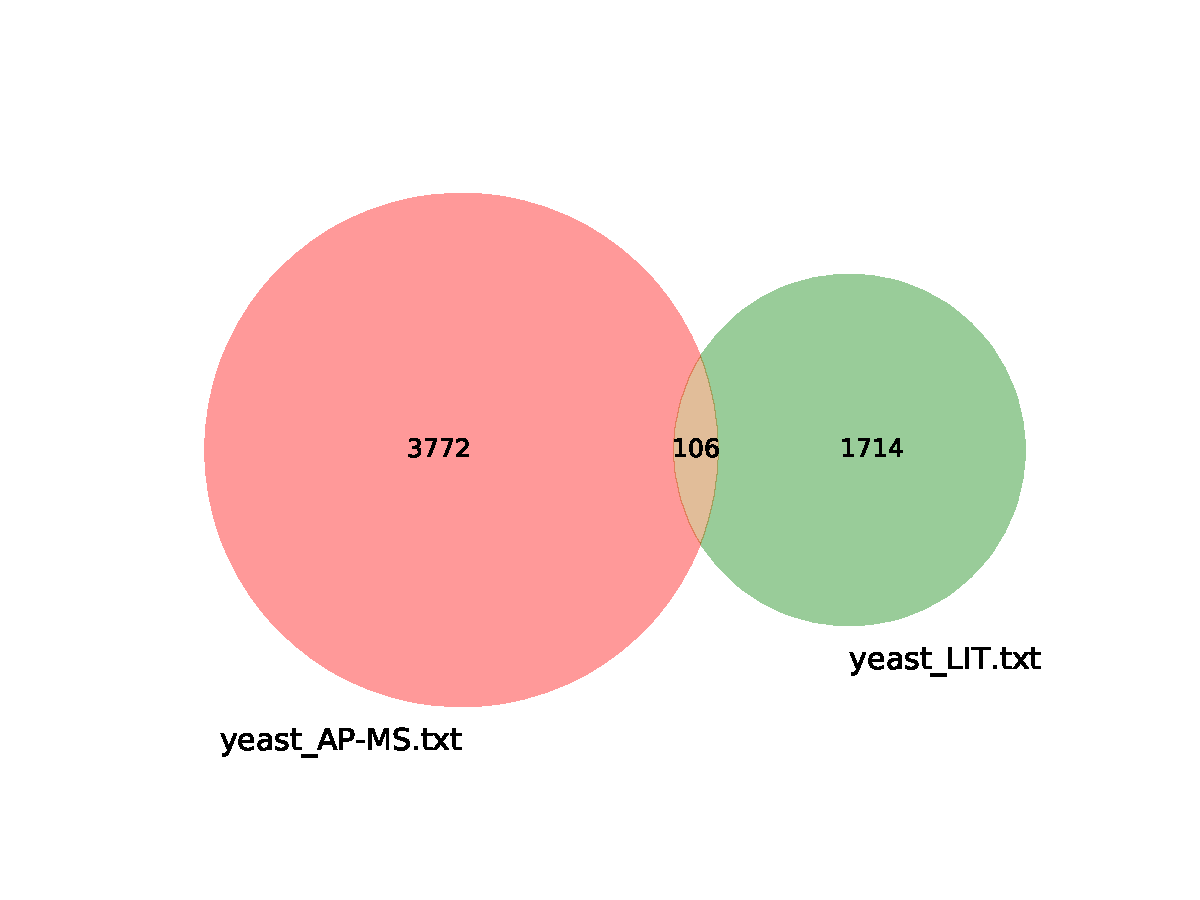
\includegraphics[width=.7\textwidth]{./schemes/venn2_coherence_yeast_AP-MS-yeast_LIT.pdf}\\
%        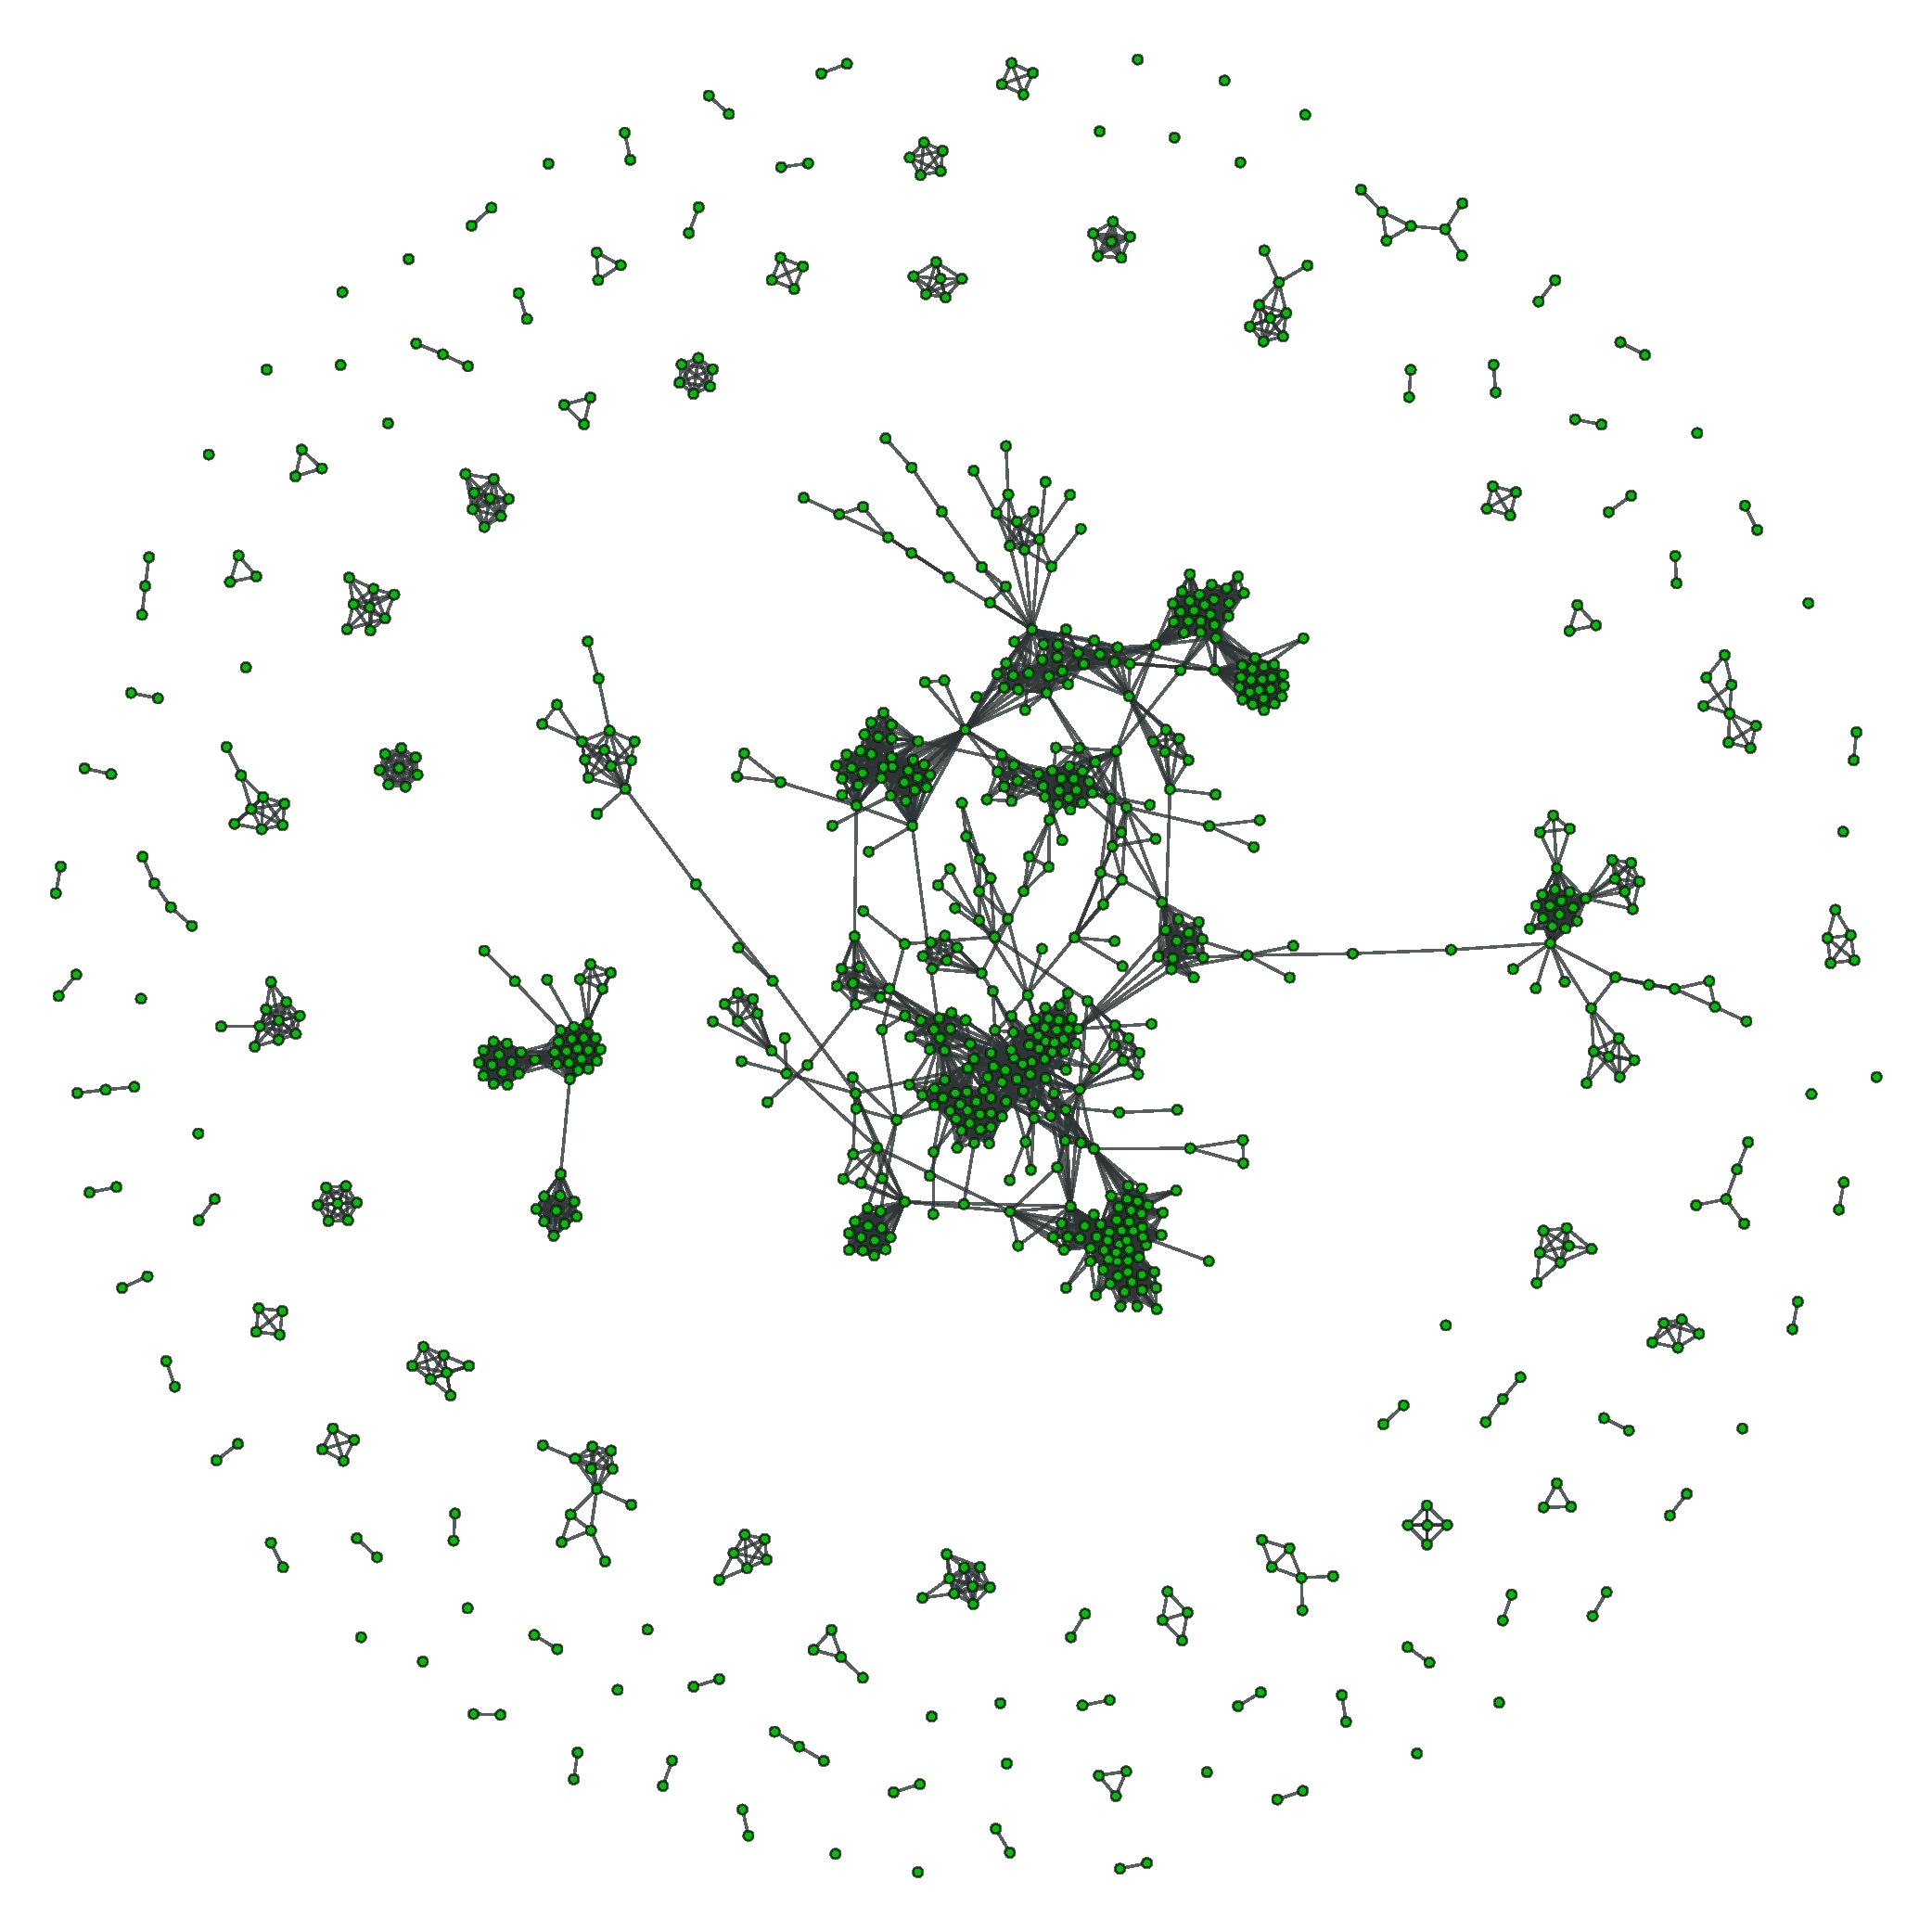
\includegraphics[width=.45\textwidth]{./schemes/subgrafo_APMS_ap_ms_lit-gml.pdf}
%        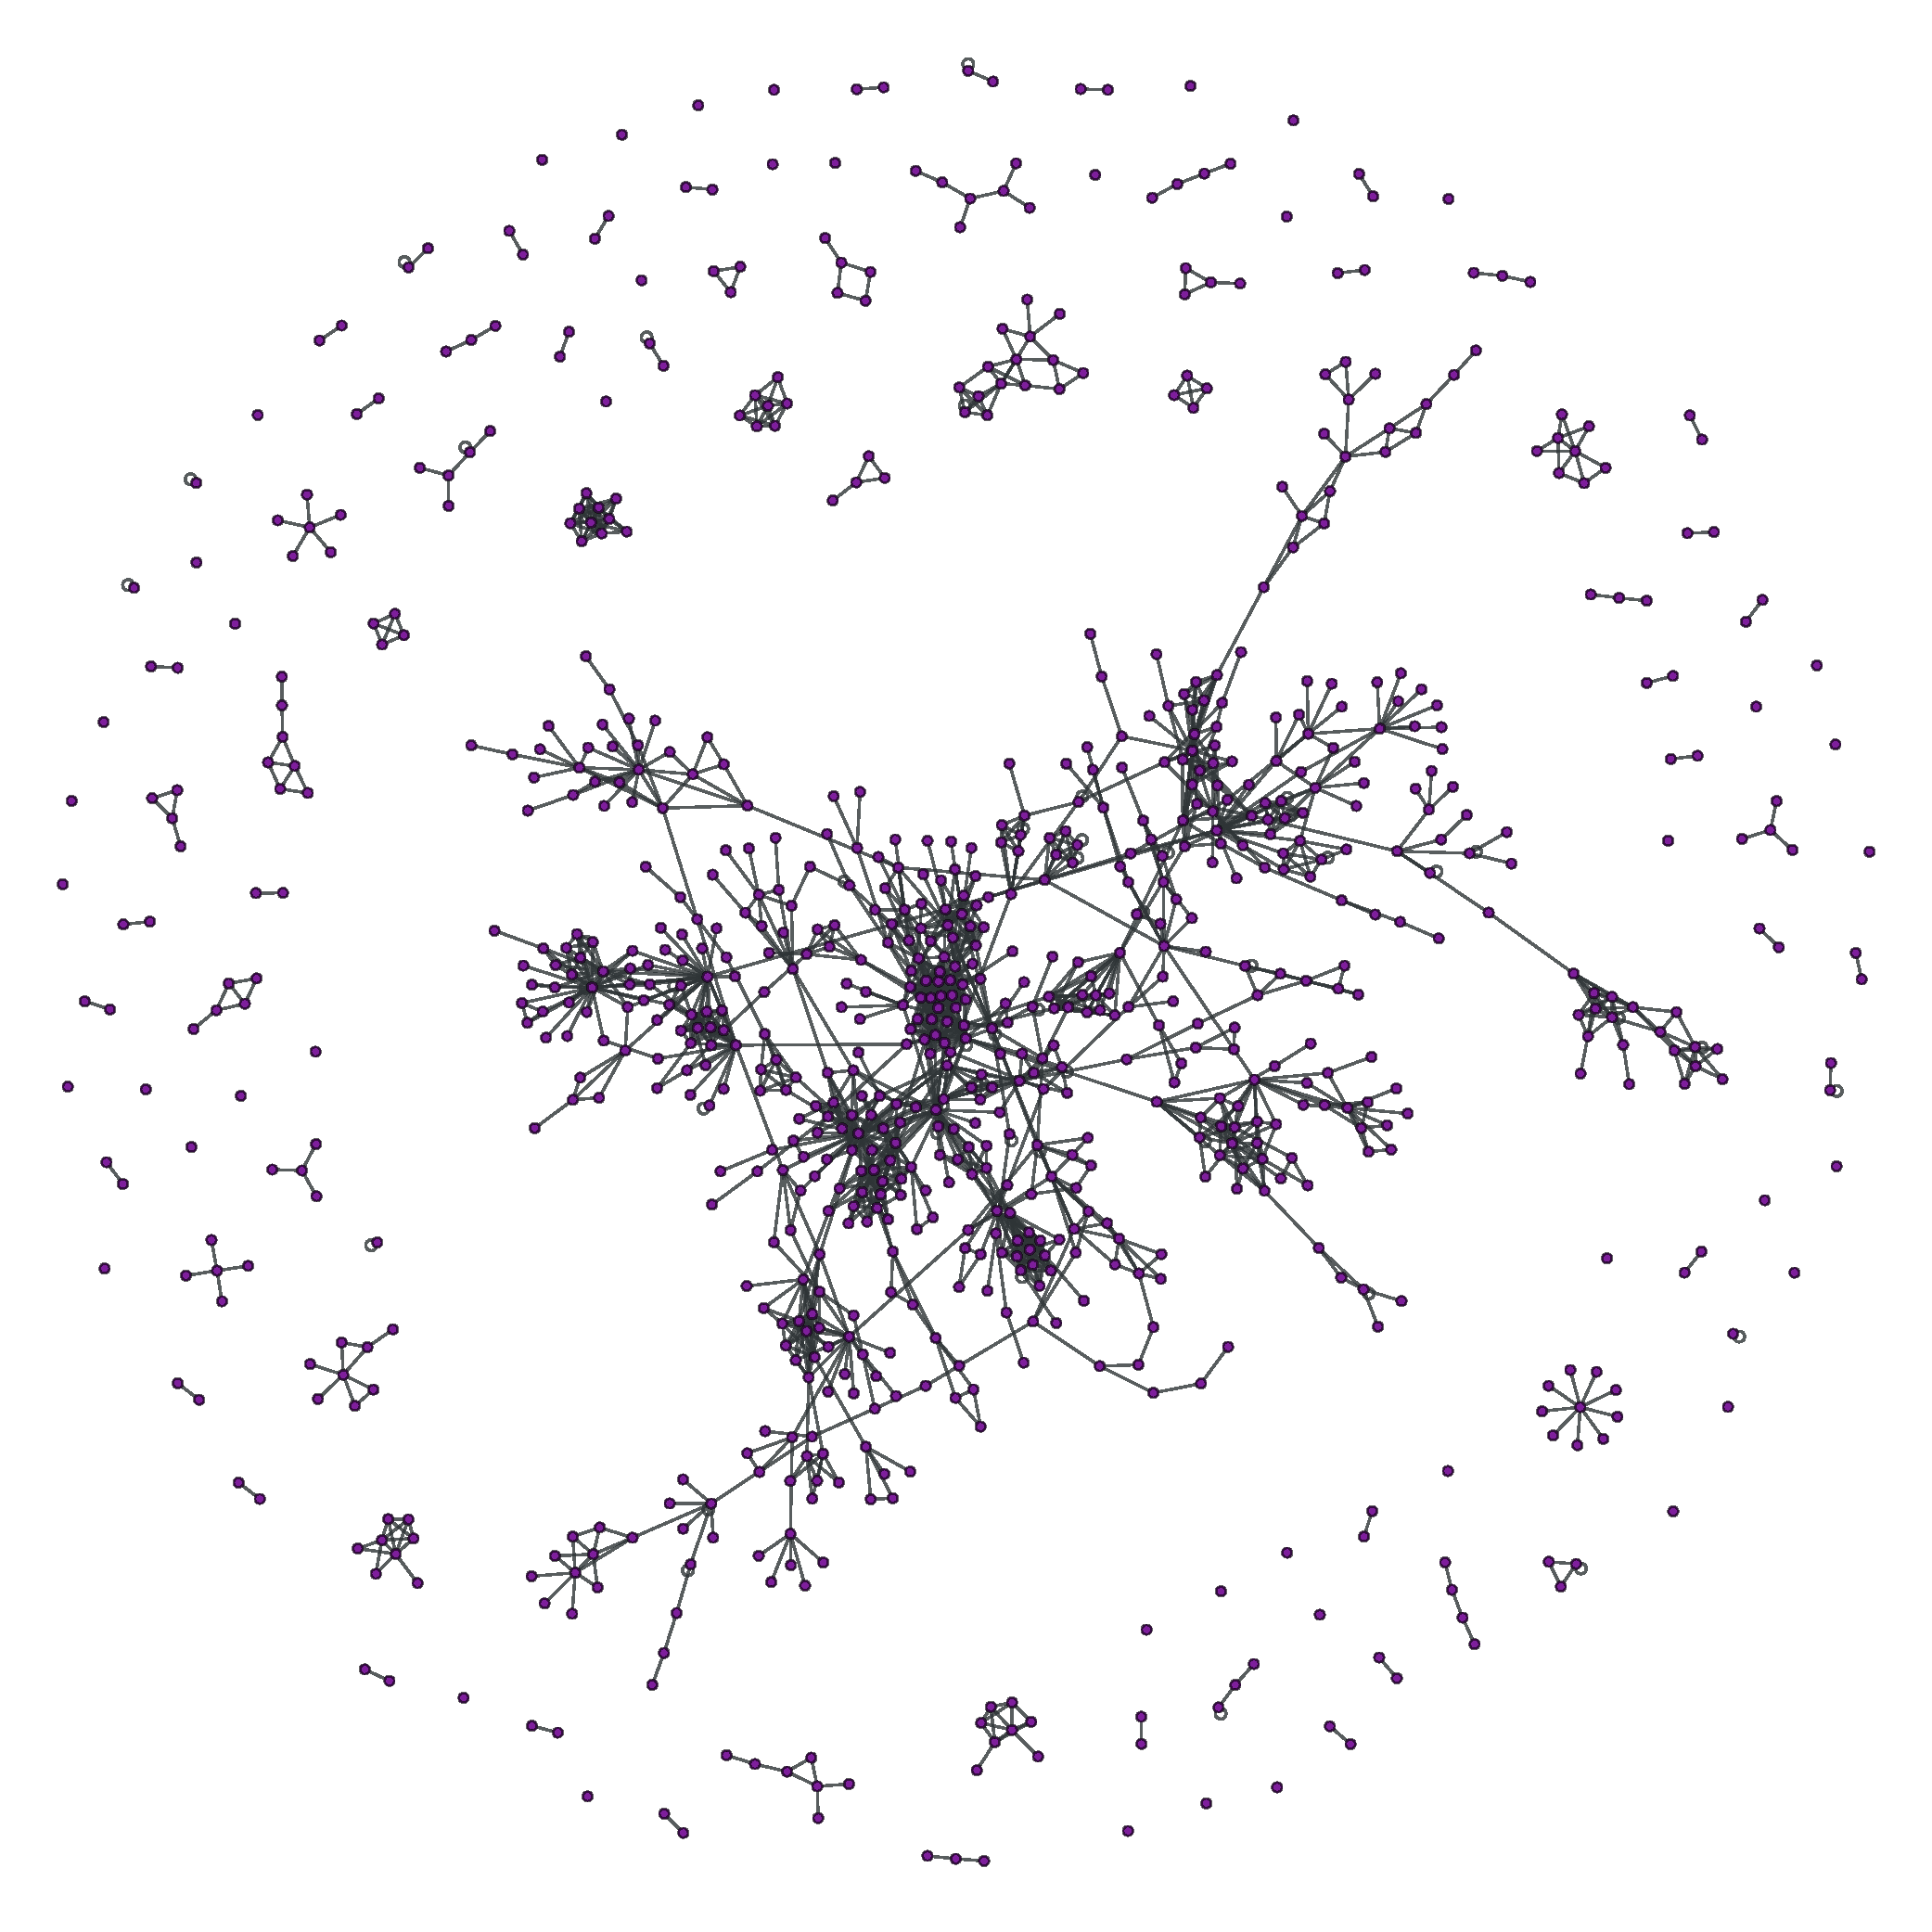
\includegraphics[width=.45\textwidth]{./schemes/subgrafo_LIT_ap_ms_lit-gml.pdf}
%        \caption{\label{fig:apms-lit} AP-MS/LIT}
%    \end{subfigure}
%    \begin{subfigure}[b]{0.3\columnwidth}
%        \centering
%        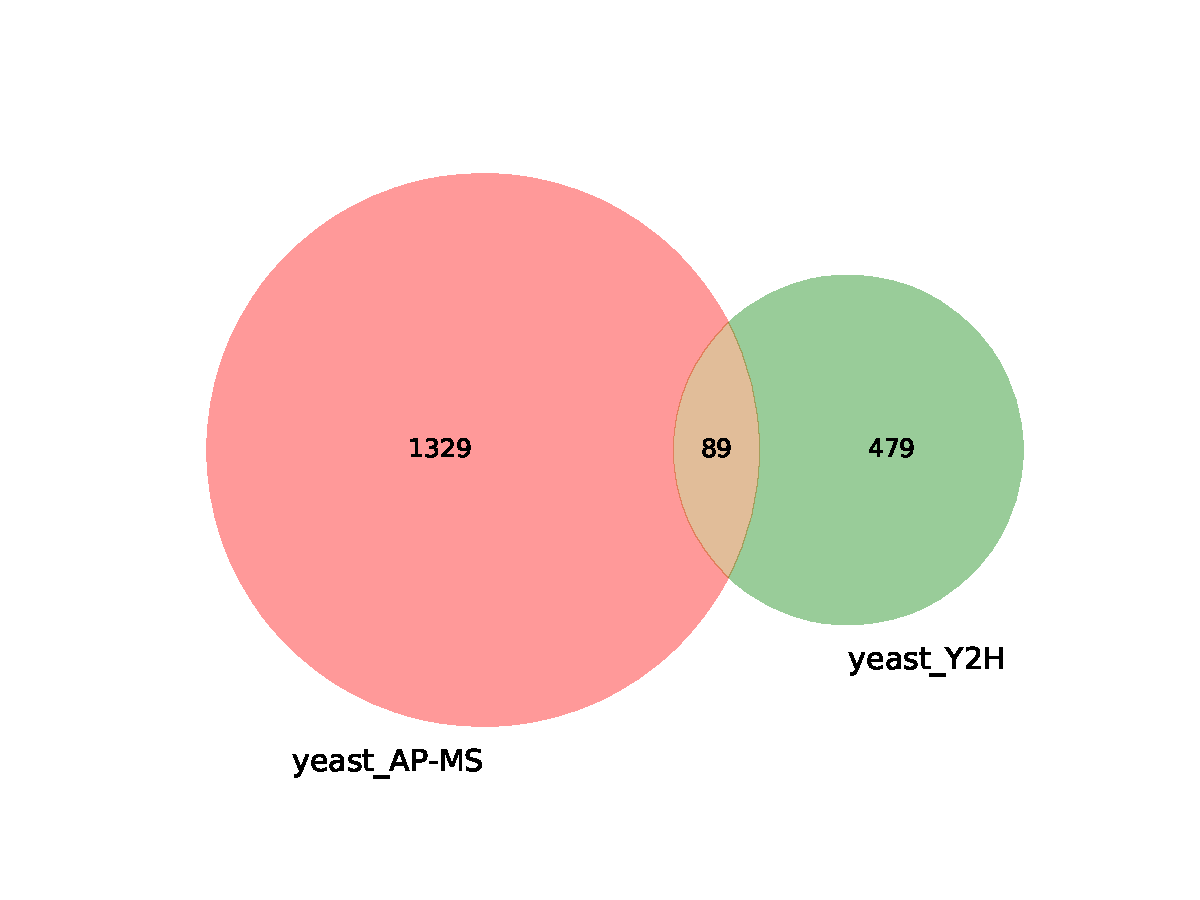
\includegraphics[width=.7\textwidth]{./schemes/venn2_coherence_yeast_AP-MS-yeast_Y2H.pdf}\\
%        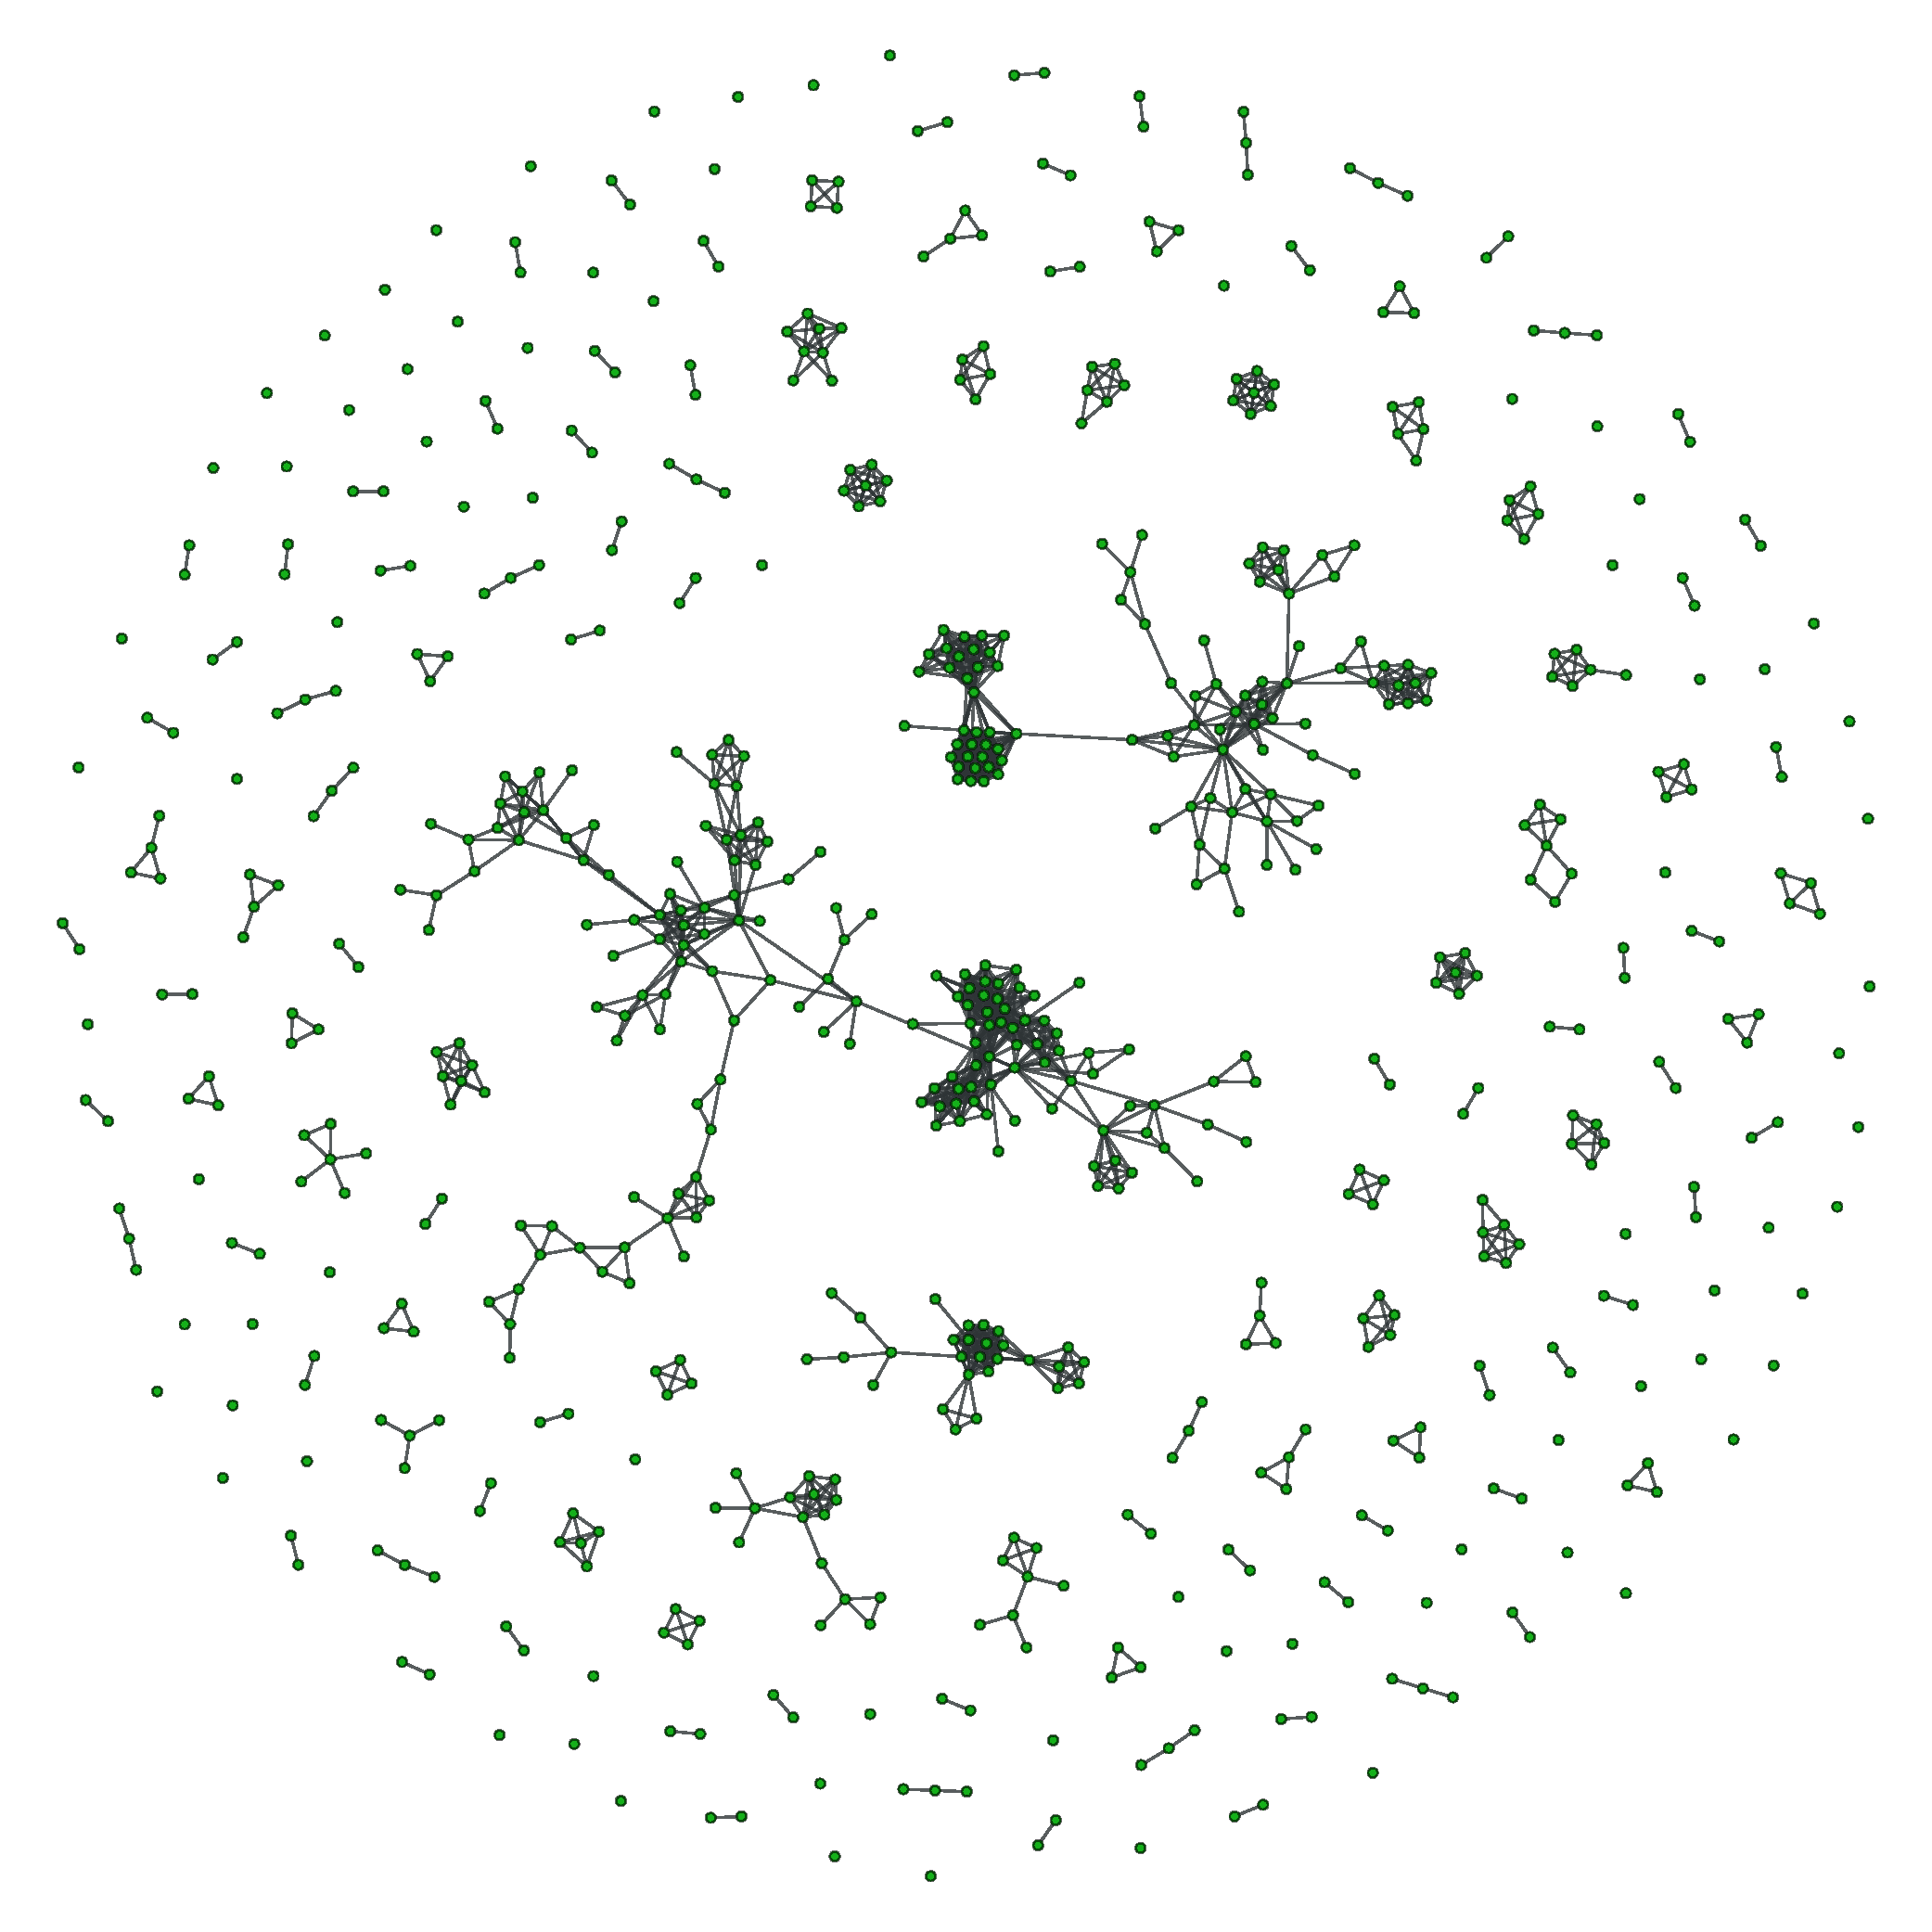
\includegraphics[width=.45\textwidth]{./schemes/subgrafo_APMS_ap_ms_y2h-gml.pdf}
%        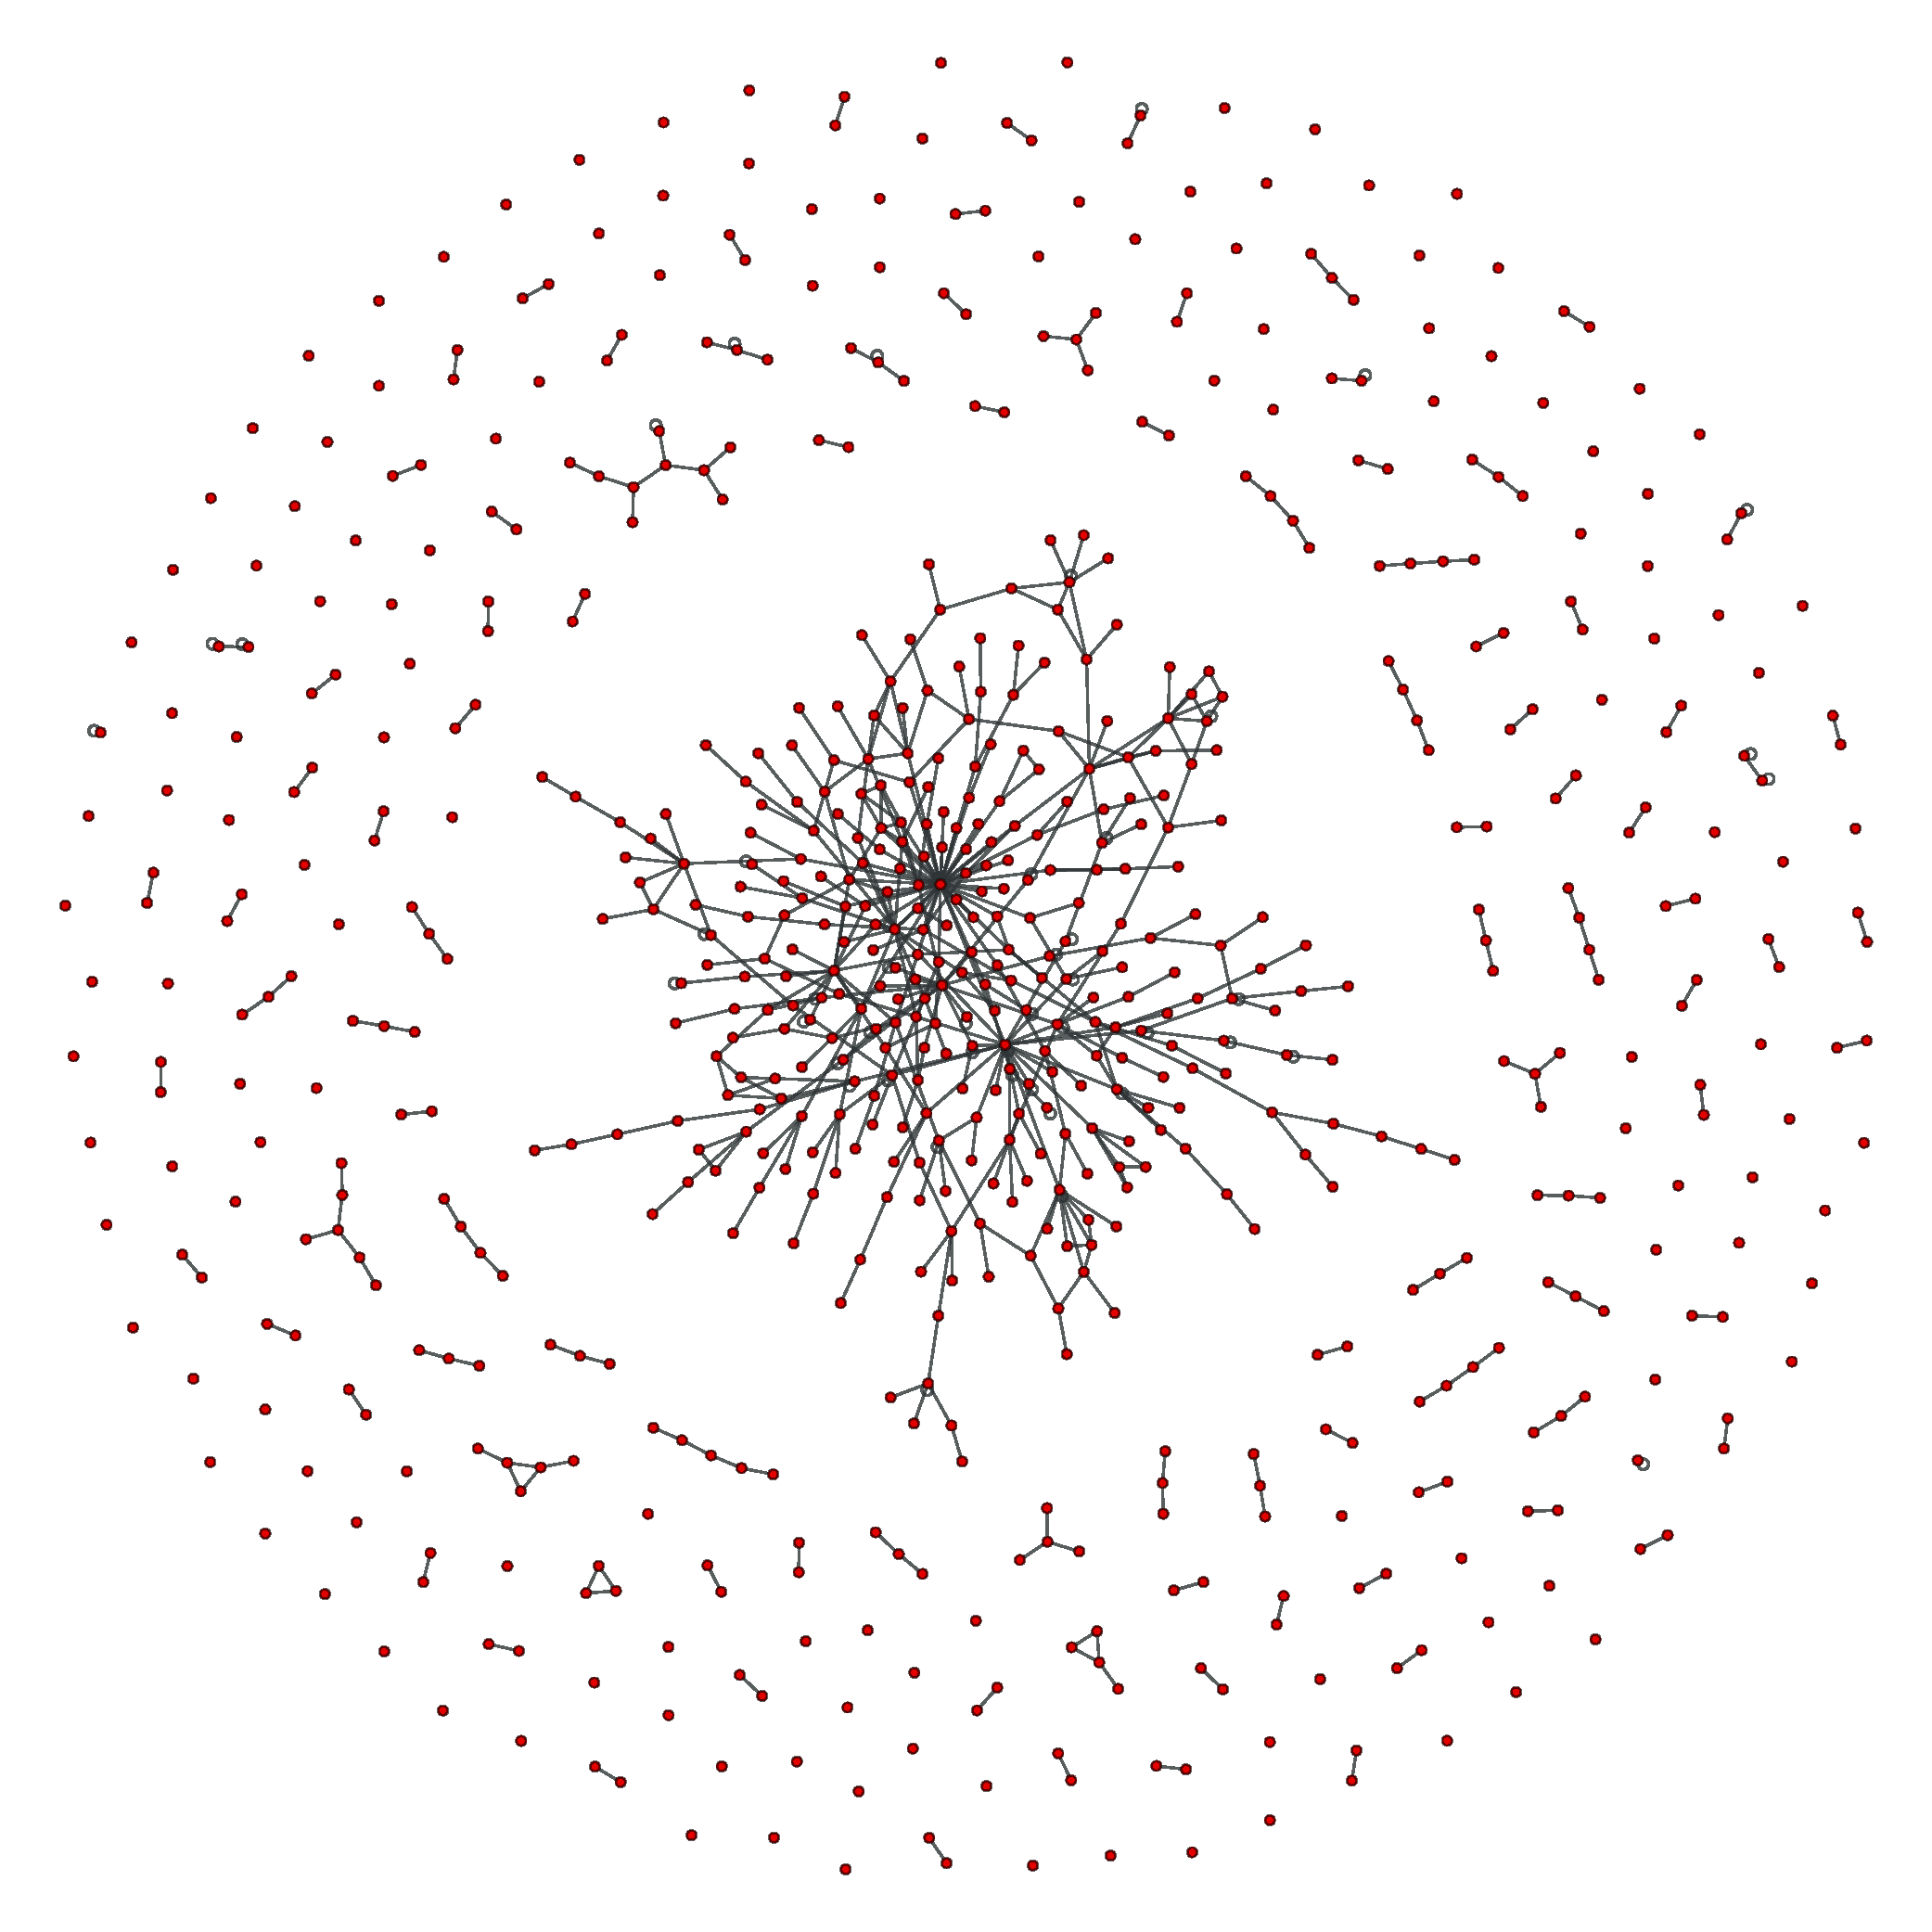
\includegraphics[width=.45\textwidth]{./schemes/subgrafo_Y2H_ap_ms_y2h-gml.pdf}
%        \caption{\label{fig:apms-y2h} AP-MS/Y2H}
%    \end{subfigure}
%    \begin{subfigure}[b]{0.3\columnwidth}
%        \centering
%        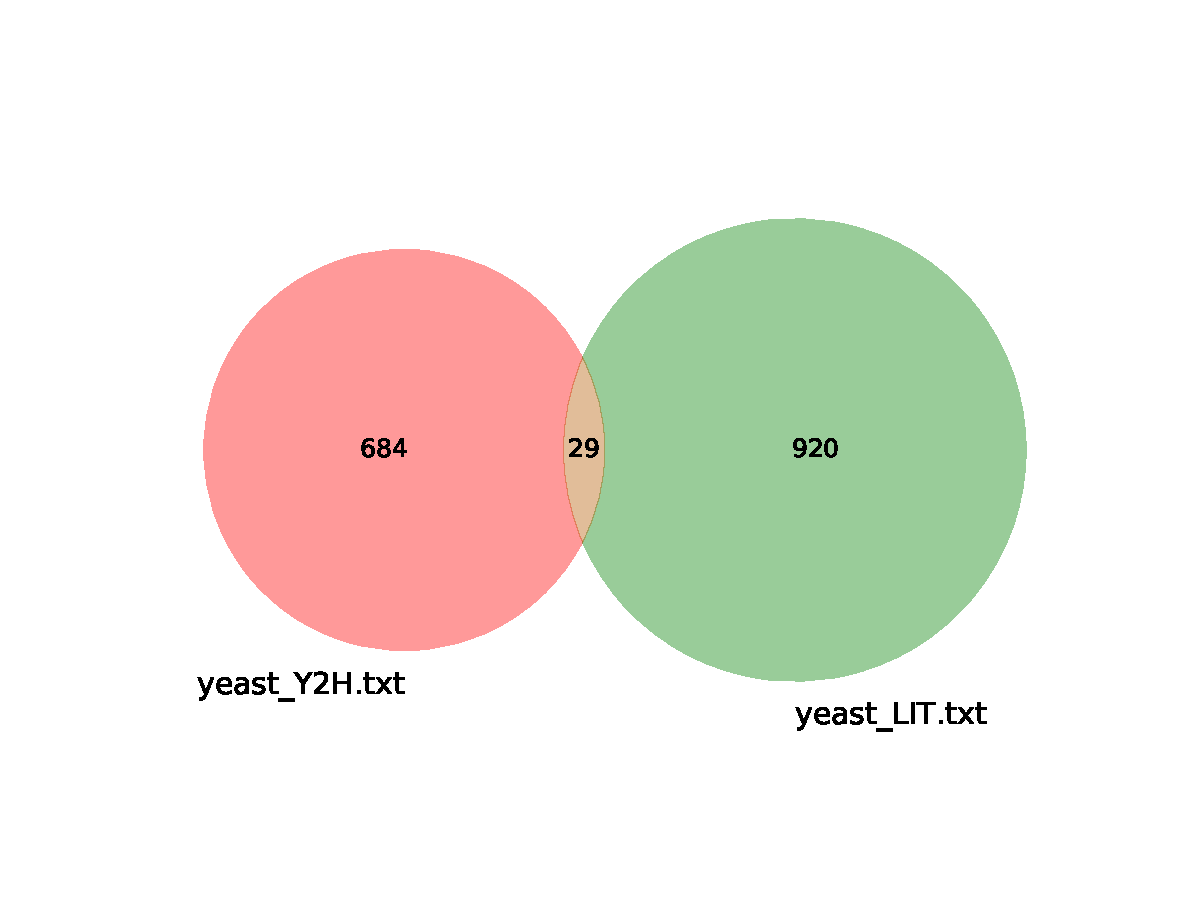
\includegraphics[width=.7\textwidth]{./schemes/venn2_coherence_yeast_Y2H-yeast_LIT.pdf}\\
%        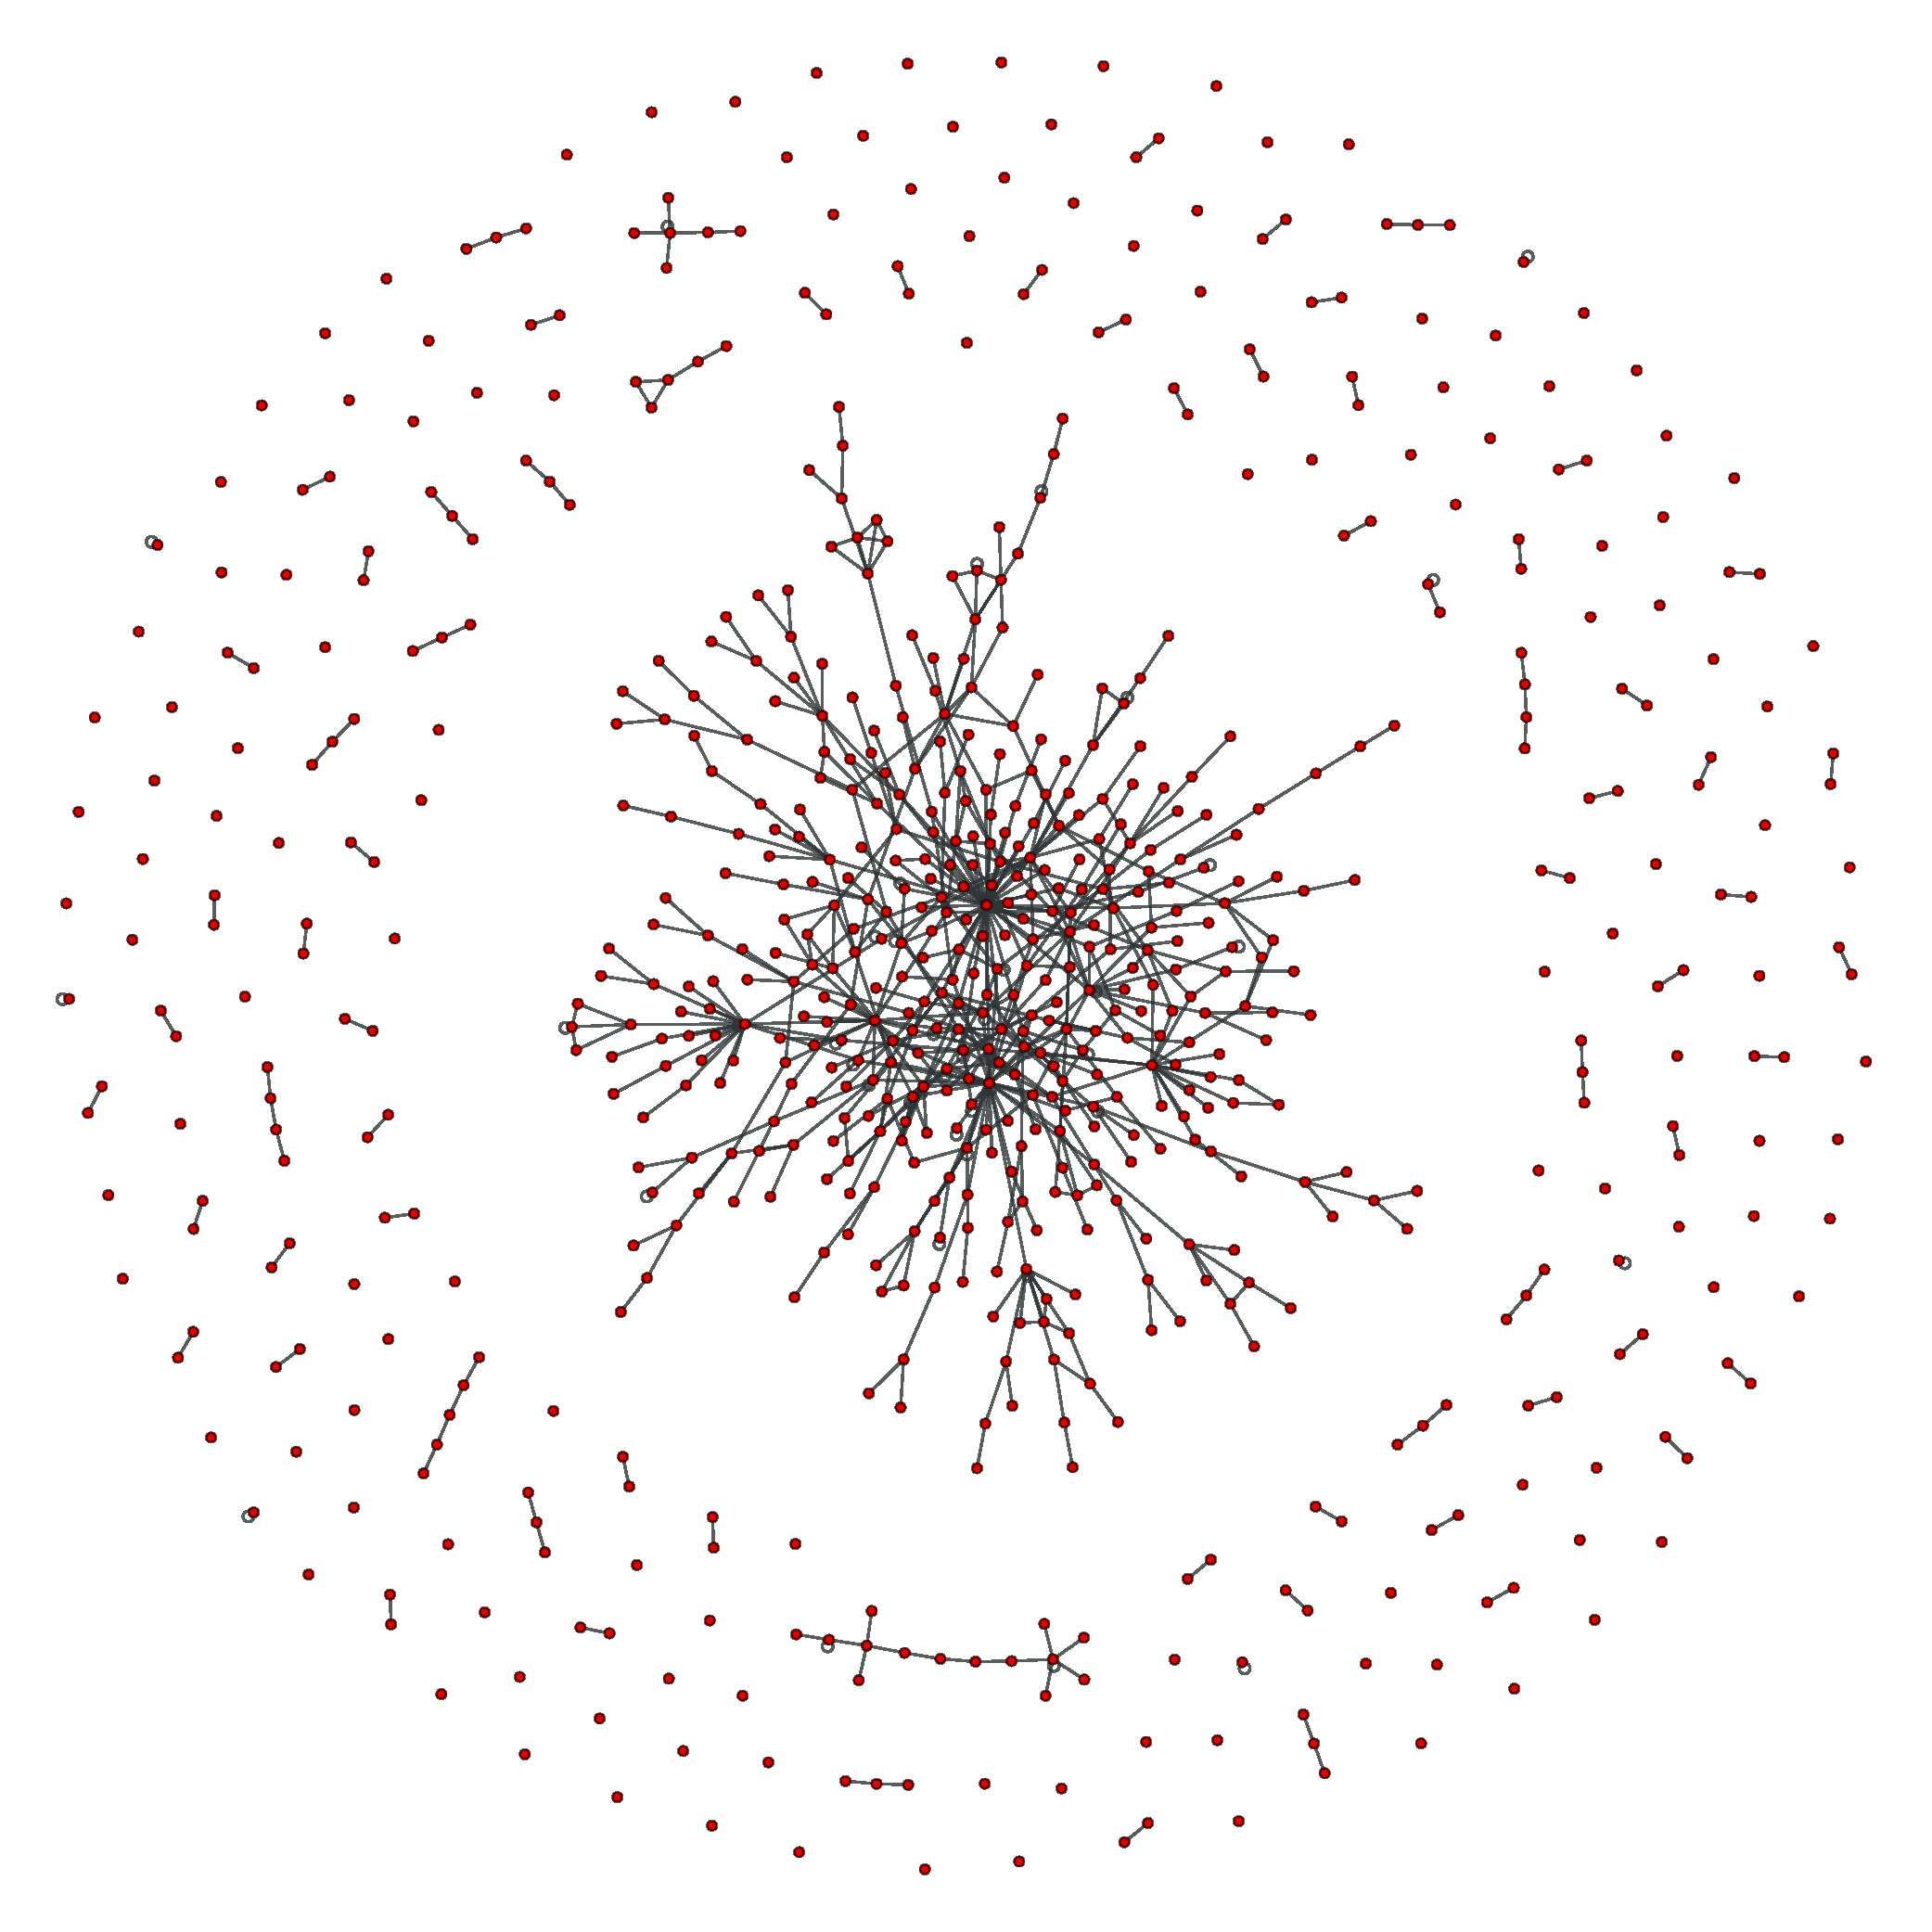
\includegraphics[width=.45\textwidth]{./schemes/subgrafo_Y2H_y2h_lit-gml.pdf}
%        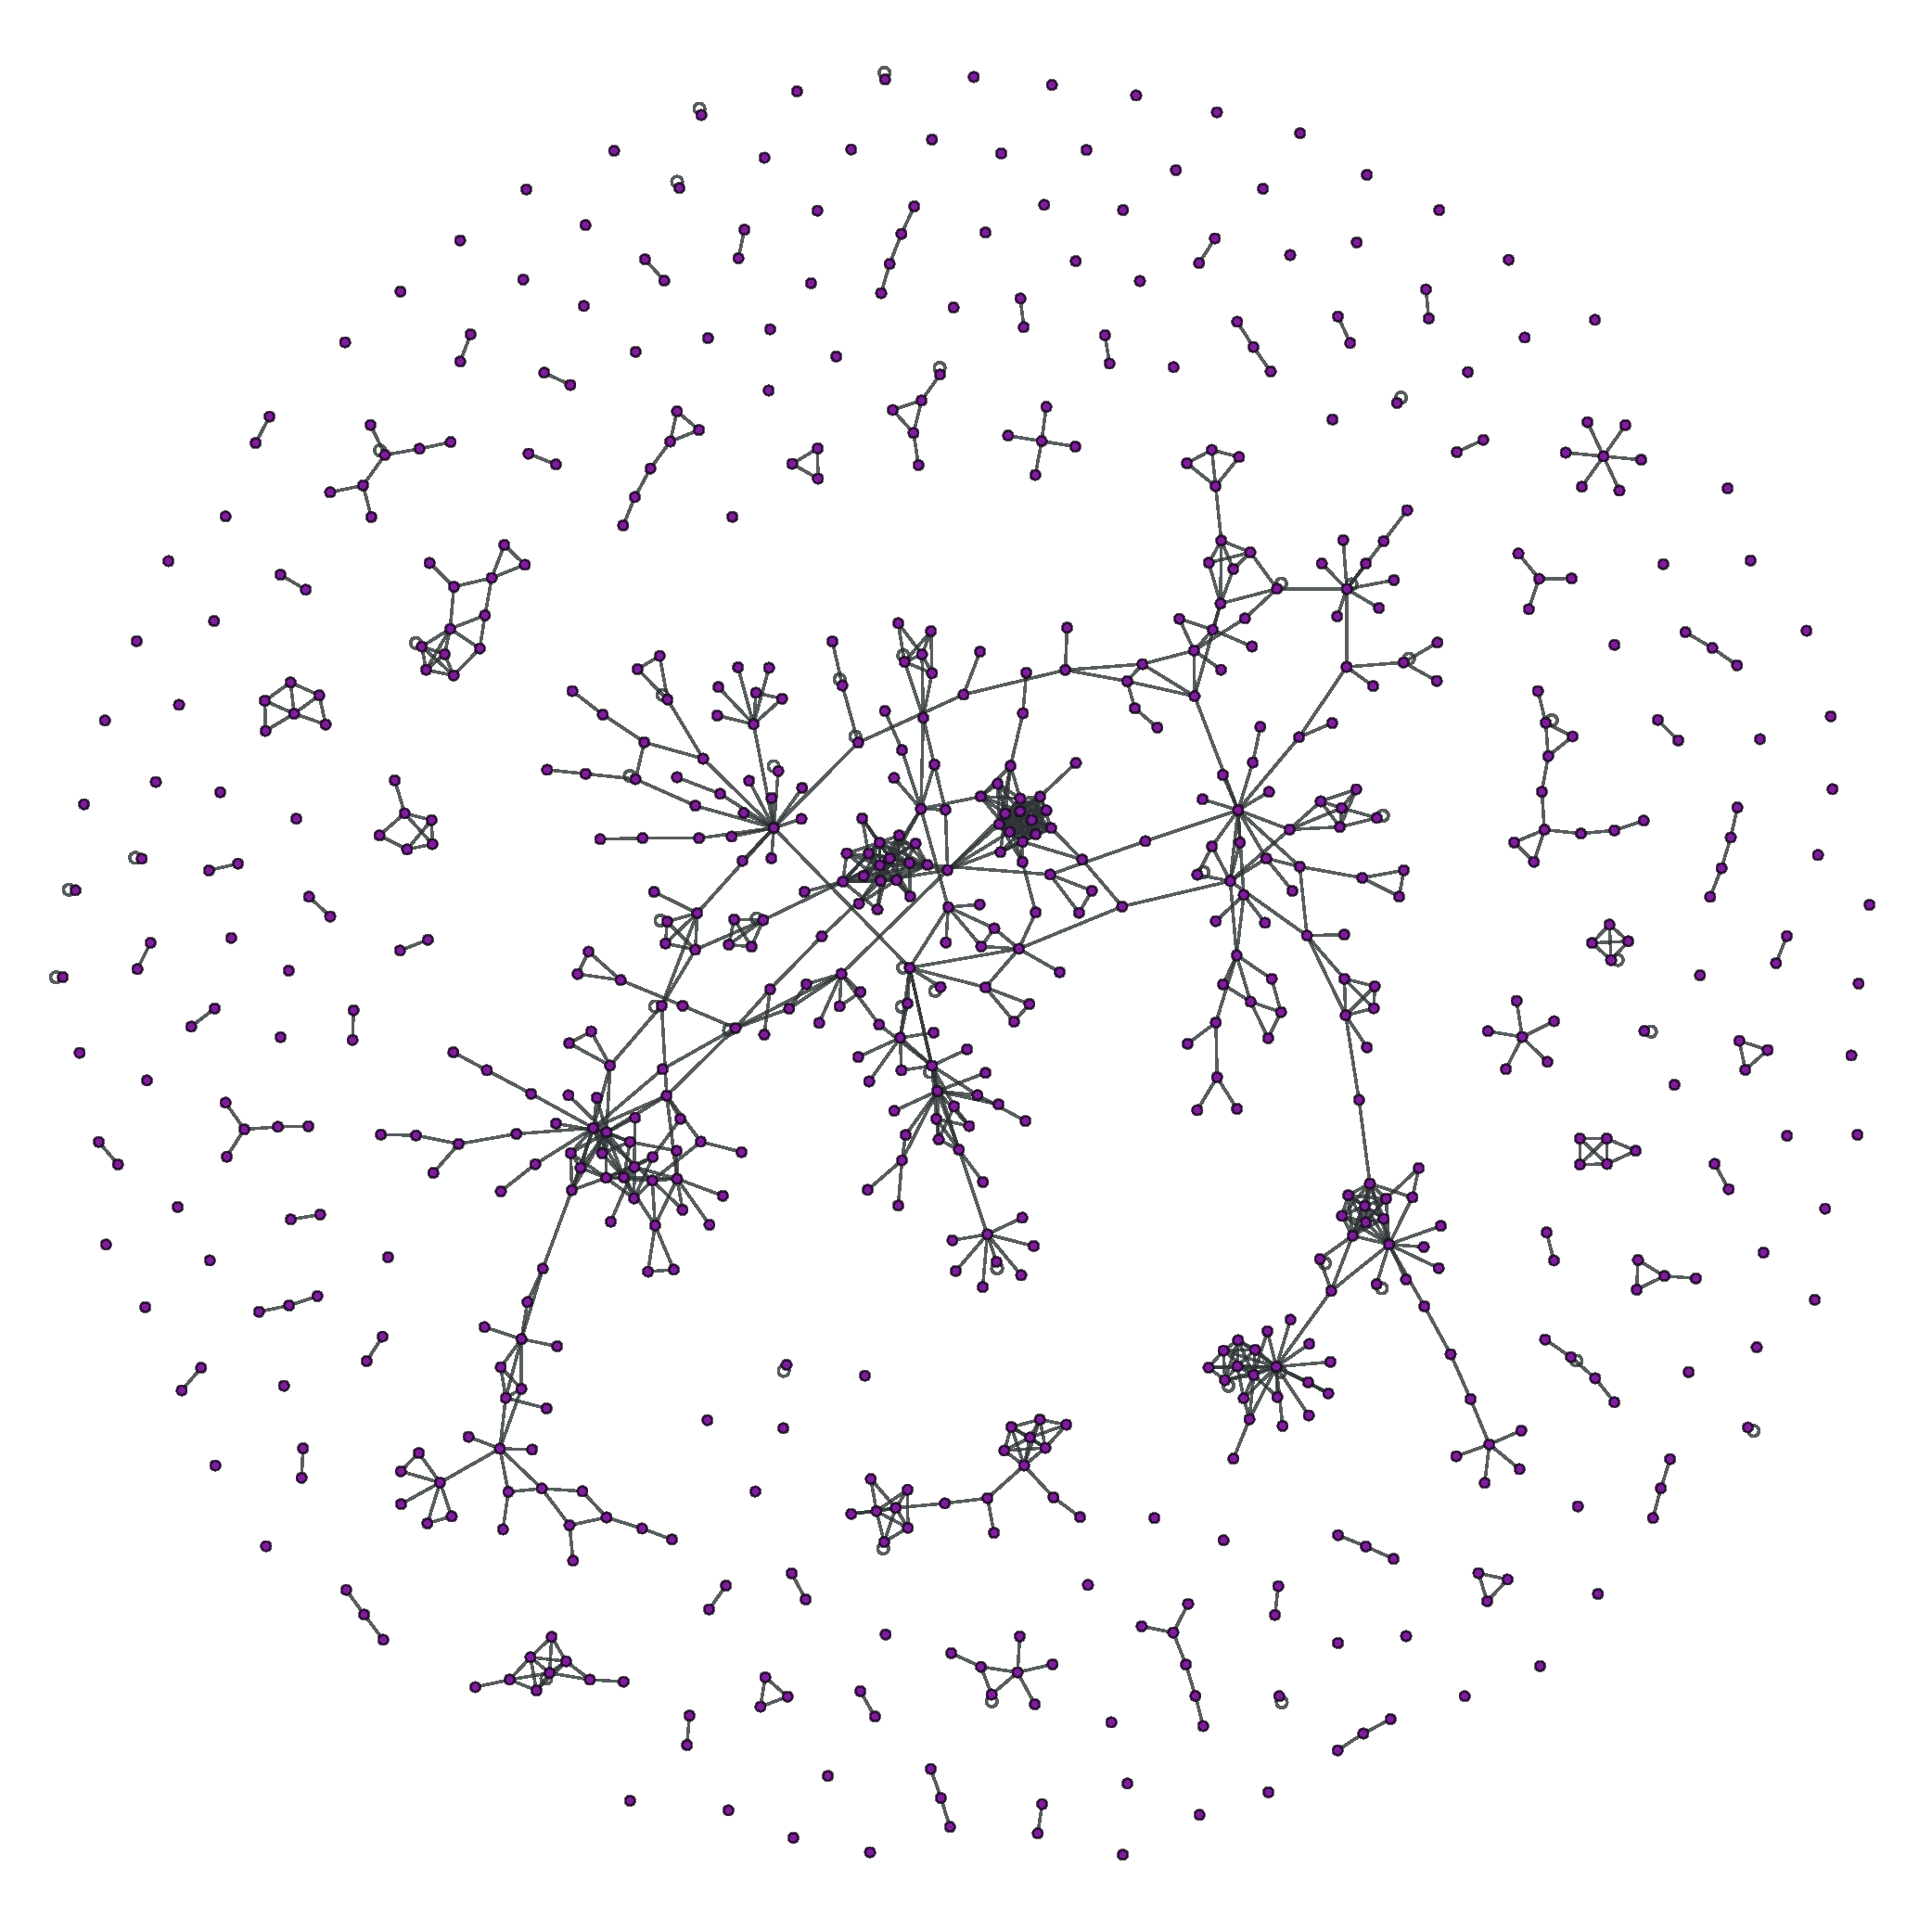
\includegraphics[width=.45\textwidth]{./schemes/subgrafo_LIT_y2h_lit-gml.pdf}
%        \caption{\label{fig:y2h-lit} Y2H/LIT}
%    \end{subfigure}
%    \caption{\label{fig:subgrafos} Coherencia entre links para cada par de redes y los respectivos subgrafos de cada red }
%\end{figure}
%
%Adicionalmente se muestran las coherencias
%a pares y los subgrafos inducidos en la figura~\ref{fig:subgrafos}. Cabe notar que, a pesar que en los subgrafos
%de la cobertura entre AP-MS y LIT podr\'ian parecer \textit{similares}, las coherencias entre links en todos los casos son
%escasas respecto a la cantidad total de links en cada subgrafo.
